%-*-coding: utf-8;-*-
\documentclass[italian,a4paper,hidelinks,headinclude]{scrartcl}
\usepackage{amsmath,amssymb,amsthm,thmtools}
\usepackage{eucal,babel,a4}
\usepackage[nochapters,pdfspacing]{classicthesis}
\usepackage[utf8]{inputenc}
\usepackage{graphicx,caption,subcaption}
\usepackage{bussproofs}
\usepackage{comment}
\usepackage{xcolor}
\usepackage{tikz,fancybox}

\newcommand{\NN}{{\mathbb N}}
\newcommand{\ZZ}{{\mathbb Z}}
\newcommand{\QQ}{{\mathbb Q}}
\newcommand{\RR}{{\mathbb R}}
\newcommand{\CC}{{\mathbb CC}}
\newcommand{\C}{{\mathcal C}}
\newcommand{\F}{{\mathcal F}}
\renewcommand{\P}{{\mathcal P}}
\newcommand{\defeq}{=}
\DeclareMathOperator{\diag}{diag}
\newcommand{\myemph}[1]{\emph{#1}\marginpar{#1}}

\newcommand{\abs}[1]{\left\vert{#1}\right\vert}
\newcommand{\enclose}[1]{\left({#1}\right)}

\renewcommand{\vec}[1]{\boldsymbol{#1}}

\def\Xint#1{\mathchoice
{\XXint\displaystyle\textstyle{#1}}%
{\XXint\textstyle\scriptstyle{#1}}%
{\XXint\scriptstyle\scriptscriptstyle{#1}}%
{\XXint\scriptscriptstyle\scriptscriptstyle{#1}}%
\!\int}
\def\XXint#1#2#3{{\setbox0=\hbox{$#1{#2#3}{\int}$ }
\vcenter{\hbox{$#2#3$ }}\kern-.6\wd0}}
\def\dashint{\Xint-}

\declaretheoremstyle[
spaceabove=6pt, spacebelow=6pt,
headfont=\normalfont\itshape,
notefont=\mdseries, notebraces={(}{)},
bodyfont=\normalfont,
postheadspace=1em,
qed=,
shaded={rulecolor=pink!30,rulewidth=1pt,bgcolor=pink!10}
]{mystyle}

\declaretheorem[numberwithin=section,name=Teorema]{theorem}
\declaretheorem[sibling=theorem,name=Definizione]{definition}
\declaretheorem[sibling=theorem,name=Lemma]{lemma}
\declaretheorem[style=mystyle,sibling=theorem,name=Esercizio]{exercise}
\declaretheorem[style=mystyle,sibling=theorem,name=Esempio]{example}
\declaretheorem[sibling=theorem,name=Paradosso]{paradox}
\declaretheorem[sibling=theorem,name=Assioma]{axiom}

\begin{document}
\title{Cenni di logica e teoria degli insiemi
\thanks{%
Puoi scaricare o contribuire a questi appunti su
\url{https://github.com/paolini/appunti/}}}
\author{E. Paolini}

\maketitle

\tableofcontents

\section{Sistemi formali}
Fin dai tempi di Aristotele si è cercato di individuare e descrivere
le leggi che governano la \emph{deduzione}. Si è osservato che
combinando tra loro singole informazioni è possibile estrarre da esse
nuove informazioni che in origine non erano disponibili. Ad esempio
dalle due informazioni
\begin{align*}
  (P) & \qquad \textit{in ogni triangolo isoscele gli angoli alla base
    sono uguali}\\
  (Q) & \qquad \textit{questo triangolo è
    isoscele}
\end{align*}
si può dedurre
\begin{align*}
  (R) \qquad \textit{gli angoli alla base di
    questo triangolo sono uguali.}
\end{align*}
Quello che abbiamo fatto è una
\emph{deduzione} (anche detta \emph{derivazione}).
Nelle notazioni dei \myemph{sistemi formali}
$P,Q,R$ si chiamano \myemph{formule}.
Una volta aggiunta $R$ alle informazioni note, si potranno fare
ulteriori derivazioni in cui oltre a $P$ e $Q$ si potrà usare anche
$R$. Questo permette di estendere l'insieme delle conoscenze, a
partire da un nucleo iniziale di conoscenze primitive che chiameremo
\myemph{assiomi}.

Le regole che ci permettono di passare da una o più formule ad una
nuova formula, si chiamano \myemph{regole di inferenza}. Normalmente le
formule sono composte da una sequenza di \myemph{simboli} che possono
essere scelti tra lettere, cifre o altro. Eventualmente una
\myemph{grammatica} determinerà come i simboli possono essere utilizzati
per comporre le formule (in tal caso le sequenze ammissibili vengono
chiamate \myemph{formule ben formate}). Le regole di inferenza
devono essere le più semplici possibile, di preferenza dovrebbero
essere delle regole \emph{meccaniche} in modo che non ci possano
essere dubbi su come vadano applicate.

Nell'esempio che abbiamo fatto all'inizio del paragrafo le formule (P), (Q) e (R)
sono espresse nel \myemph{linguaggio naturale} ovvero nella lingua che
siamo abituati ad utilizzare ogni giorno. Formalizzare il linguaggio
naturale risulta un compito improbo: sono troppe le ambiguità, i
sottointesi, le interpretazioni soggettive, perché si possa pensare di
trovare le regole di inferenza di tale linguaggio. Quello che si può fare è
costruire un \myemph{linguaggio artificiale} che sia  sufficientemente
semplice da poter essere formalizzato in modo non ambiguo
e sufficientemente complesso per ottenere delle derivazioni non banali che possano avere utilità pratica.

 Normalmente
il linguaggio artificiale sarà comunque ispirato al linguaggio
naturale. E' però possibile costruire dei linguaggi che non abbiano
niente a che fare con la lingua naturale, e questo può essere un utile
esercizio perché ci mette nella situazione di non poter dare un significato
alle formule e di doversi quindi ciecamente e meccanicamente affidare
alle regole formali di inferenza. Lo facciamo nel seguente
esempio\footnote{%
  Esempio tratto dal libro
    \emph{G\"odel, Escher, Bach: un'eterna ghirlanda brillante} di
    Douglas Hofstadter}.

\begin{example}[sistema \texttt{MIU}]
Prendiamo come simboli le lettere: \texttt{MIU}.
Consideriamo ben formate tutte
le formule composte da una sequenza di queste lettere. Ad esempio
saranno formule ben formate: \texttt{UMI, MIMMI, IMMUMMMIIUMI}. Come
regole di inferenza consideriamo le seguenti:
\begin{enumerate}
\item  $x$\texttt{I} $\to$ $x$\texttt{IU} (cioé: si può aggiungere una
  \texttt{U} alla fine delle formule che terminano con \texttt{I})
\item \texttt{M}$x$ $\to$ \texttt{M}$xx$ (cioé: si può raddoppiare la
  sequenza di simboli dopo una \texttt{M} iniziale)
\item $x$\texttt{III}$y$ $\to$ $x$\texttt{U}$y$ (cioé: si può
  rimpiazzare ogni sequenza \texttt{III} con \texttt{U})
\item $x$\texttt{UU}$y$ $\to$ $xy$ (cioé: si può rimuovere la sequenza \texttt{UU}).
\end{enumerate}
Ecco un esempio di derivazione a partire dalla formula \texttt{MIIMI}:
\begin{center}
  \begin{tabular}{l}
    \texttt{MIIMI} (ipotesi)\\\hline
    \texttt{MIIMIIIMI} (regola 2.)\\
    \texttt{MIIMUMI} (regola 3.)\\
    \texttt{MIIMUMIU} (regola 1.)\\
  \end{tabular}
\end{center}

A partire dalla formula \texttt{MI} è possibile derivare la formula \texttt{MU}?
\end{example}

\marginpar{sistema \texttt{IVXPU}}
\begin{example}
Si  considerino le formule formate dai simboli
\texttt{IVXPU}.
Si prendano le seguenti regole di inferenza:
  \begin{enumerate}
  \item $x$\texttt{P}$y$\texttt{U}$z$ $\to$ $x$\texttt{IP}$y$\texttt{U}$zy$,
  \item $x$\texttt{P}$y$\texttt{U}$z$ $\to$ $x$\texttt{P}$y$\texttt{IU}$zx$,
  \item $x$\texttt{IIIII}$y$ $\to$ $x$\texttt{V}$y$,
  \item $x$\texttt{VV}$y$ $\to$ $x$\texttt{X}$y$.
  \end{enumerate}
  Si prenda come assioma: \texttt{IPIUI}. Si riesce ad ottenere la formula \texttt{VPVUXXV}?
\end{example}

Per risolvere la richiesta precedente probabilmente è
necessario trovare una \emph{interpretazione} dei simboli
utilizzati. Si provi a immaginare che i simboli \texttt{IVX}
rappresentino numeri romani... come vanno interpretati i simboli
\texttt{PU} per dare un senso comune alle formule del sistema
\texttt{IVXPU}?

\section{Modello, verità, completezza}

Nel sistema formale \texttt{IVXPU}
che abbiamo considerato nel paragrafo precedente i simboli possono essere interpretati
come operazioni su numeri naturali. Si dice allora che l'insieme dei
numeri naturali fornisce un \myemph{modello} per questo sistema
formale. Il modello associa un valore di \myemph{verità} ad ogni formula.
Se ogni assioma viene interpretato come un fatto vero, e ogni regola
formale mantiene il valore di \emph{verità} delle formule (cioè
partendo da una formula vera e applicando una qualunque regola formale
si ottiene un'altra formula vera) allora ogni derivazione del sistema
formale produce sicuramente formule vere.

Nel nostro caso l'assioma \texttt{IPIUI} corrisponde alla verità:
$1\cdot 1 = 1$ e
la prima regola di inferenza corrisponde alla seguente verità:
\[
\text{se $x\cdot y = z$ allora $(x+1)\cdot y = z + y$.}
\]
E' dunque chiaro che ogni formula ottenuta con questo sistema formale
sarà interpretata come vera. Ci chiediamo: è possibile, in questo
sistema, derivare qualunque formula vera? La risposta è negativa
in quanto si può osservare che la formula: \texttt{VIUIIIPII} potrebbe
essere interpretata come $6 = 3\cdot 2$ che è vera, ma non può essere
dimostrata mediante le regole formali che abbiamo scelto.
In questo caso si dice che il sistema è \myemph{incompleto} in quanto ci sono
formule vere che non possono essere dimostrate.

Si potrebbero aggiungere delle regole \emph{grammaticali}
per mettere dei vincoli su quali siano le formule ben formate. Si
potrebbe ad esempio richiedere che la formula contenga una sola
\texttt{P} e una sola \texttt{U} e che la \texttt{P} si trovi sempre
prima della \texttt{U}. In questo modo si escludono tutte le formule
vere che non posso essere derivate e il sistema si dice \emph{completo}.
Il concetto di \myemph{completezza} è fondamentale per capire il significato
del teorema di G\"odel, di cui parleremo brevemente più avanti.





\section{Logica delle proposizioni}

Nella \emph{logica delle proposizioni} si aggiunge il concetto di
\emph{verità} all'interno del sistema formale.
Le formule prendono il nome di \myemph{proposizioni} e possono assumere un valore
di verità:
\texttt{V}=\myemph{vero} o \texttt{F}=\myemph{falso}.
Si introducono quindi i \myemph{connettivi logici} ovvero gli operatori
$\neg$ (negazione: non), $\land$ (congiunzione: e), $\lor$ (disgiunzione:
o), $\Rightarrow$ (implicazione: solo se), $\Leftarrow$ (implicazione
inversa: se), $\Leftrightarrow$ (doppia implicazione: se e solo se) che
applicati ad una (per la negazione) o due proposizioni (per tutti gli altri
connettivi) producono una nuova proposizione il cui valore di verità
può essere meccanicamente dedotto dal valore di verità delle
proposizioni a cui è stato applicato. Essendoci solo un numero finito di
combinazioni, possiamo definire le operazioni logiche elencando, in
forma di tabella, tutti i valori possibili che possono assumere una
coppia di proposizioni $P$ e $Q$ e i corrispondenti valori per le
varie operazioni riferite a $P$ e $Q$:

\medskip

\begin{center}
  \begin{tabular}{cc|cccccc}
    $P$ & $Q$ & $\neg P$ & $P\land Q$ & $P\lor Q$ & $P\Rightarrow Q$ &
    $P\Leftarrow Q$ & $P\Leftrightarrow Q$ \\\hline
    \texttt{V} & \texttt{V} & \texttt{F} & \texttt{V} & \texttt{V} & \texttt{V} & \texttt{V} & \texttt{V} \\
    \texttt{V} & \texttt{F} & \texttt{F} & \texttt{F} & \texttt{V} & \texttt{F} & \texttt{V} & \texttt{F} \\
    \texttt{F} & \texttt{V} & \texttt{V} & \texttt{F} & \texttt{V} & \texttt{V} & \texttt{F} & \texttt{F} \\
    \texttt{F} & \texttt{F} & \texttt{V} & \texttt{F} & \texttt{F} & \texttt{V} & \texttt{V} & \texttt{V} \\
    \end{tabular}
\end{center}

I valori assegnati in questa tabella sono ispirati al significato
delle corrispondenti particelle del linguaggio naturale. Si scoprirà,
tuttavia, che nel linguaggio naturale le particelle corrispondenti ai
connettivi logici hanno una interpretazione che in molti casi dipende
dal contesto e che è quindi molto più complessa e ambigua di quanto
non sia il corrispondente connettivo logico. Ma è proprio per evitare
le ambiguità e per rendere la verifica di una derivazione un fatto
puramente meccanico indipendente dal significato (o \myemph{semantica})
delle proposizioni coinvolte, che abbiamo introdotto i linguaggi
formali.

Alcuni esempi in cui il linguaggio formale si discosta
dall'interpretazione puramente meccanica: ``non ho visto niente''
(la doppia negazione dovrebbe elidersi), ``caffé o cappuccino?''
(escludendo la possibilità di scegliere entrambi). L'implicazione
logica è probabilmente una delle operazioni che possono sembrare più
controverse per quanto riguarda le ultime due righe della tabella che
affermano la verità di \texttt{F}$\Rightarrow$\texttt{V} e di
\texttt{F}$\Rightarrow$\texttt{F} (da un fatto falso segue qualunque
cosa o \emph{ex falso quodlibet}). Per convincerci che in effetti la
scelta di questi valori di verità è quella \emph{giusta}, si consideri
come esempio
la seguente implicazione:
\[
n > 5 \Rightarrow n > 3
\]
che si può leggere: ``se un numero è maggiore di 5 allora è anche
maggiore di 3''. Siamo convinti che questa implicazione debba essere vera comunque
venga scelto il numero $n$. Scegliendo per $n$ i valori $7$, $4$ e $2$
si ottengono allora le seguenti implicazioni
\[
7 > 5 \Rightarrow 7>3, \qquad 4>5 \Rightarrow 4 > 3, \qquad 2>5
\Rightarrow 2>3
\]
che diventano rispettivamente:
\[
\texttt{V} \Rightarrow \texttt{V}, \qquad
\texttt{F} \Rightarrow \texttt{V}, \qquad
\texttt{F} \Rightarrow \texttt{F}
\]
che sono quindi tutte e tre implicazioni vere, coerentemente con
quanto riportato nella tabella.

Combinando tra loro più operazioni logiche, si potranno
aggiungere altre colonne alla tabella già vista, arrivando facilmente
ad ottenere tutte le possibili 16 combinazioni di valori di verità. Ad
esempio si potrebbe introdurre la disgiunzione esclusiva (\emph{xor})
con la seguente espressione: $(P \lor Q) \land \neg (P\land Q)$ (che
si interpreta come: $P$ o $Q$ ma non entrambi) la cui colonna di
valori di verità risulta essere $\texttt{FVVF}$. Essendoci solamente
un numero finito di possibili valutazioni di una espressione logica, è
utile sapere che ogni espressione molto lunga potrà essere certamente
semplificata. Le regole più utili che permettono di manipolare le
espressioni logiche sono quelle elencate nella Tabella~\ref{tab:operatori_logici}.
Tutte le righe della tabella possono essere verificate
osservando che comunque vengano assegnati dei valori di verità alle proposizioni
$P$, $Q$ ed $R$ si ottiene una proposizione vera (sono, cioè, delle tautologie).


\medskip

\begin{table}
\begin{tabular}{rcll}
                         $\neg \neg P$ & $\iff$ & $ P$                           & doppia negazione\\
                                    $P \land Q$ & $\iff$ & $ Q \land P$                   & simmetria\\
                                     $P \lor Q$ & $\iff$ & $ Q \lor P$                    & \\
                              $\neg (P\land Q)$ & $\iff$ & $ (\neg P) \lor (\neg Q)$      & formule di De Morgan\\
                               $\neg (P\lor Q)$ & $\iff$ & $ (\neg P) \land (\neg Q)$     & \\
                            $(P\land Q) \lor R$ & $\iff$ & $ (P\lor R) \land (Q \lor R)$  & proprietà distributiva\\
                            $(P\lor Q) \land R$ & $\iff$ & $ (P\land R) \lor (Q \land R)$ & \\
                            $(P \Rightarrow Q)$ & $\iff$ & $ (Q \Leftarrow P)$            & antisimmetria\\
  $((P \Rightarrow Q) \land (Q \Rightarrow P))$ & $\iff$ & $ (P \Leftrightarrow Q)$       & doppia implicazione\\
                        $\neg (P\Rightarrow Q)$ & $\iff$ & $ P \land (\neg Q)$            & controesempio\\
                             $(P\Rightarrow Q)$ & $\iff$ & $ (\neg Q\Rightarrow\neg P)$   & implicazione contropositiva\\
                             $P$                & $\Longrightarrow$& $ (Q \Rightarrow P \wedge Q)$  & introduzione congiunzione\\
                             $P$                & $\Longrightarrow$& $ P \vee Q $                   & introduzione disgiunzione
\end{tabular}
\caption{Proprietà degli operatori logici}
\label{tab:operatori_logici}
\end{table}
\medskip

Un esempio di implicazione logica tratta dal linguaggio naturale è la
seguente ``non aprire se non in caso di pericolo'' (si può trovare
scritta sul meccanismo manuale di apertura delle porte di un treno).
Questa frase ha la struttura $(\neg P) \Leftarrow (\neg Q)$ dove $P$
rappresenta ``aprire'' e $Q$ rappresenta ``in caso di
pericolo''. Passando alla \emph{contropositiva} la proposizione
risulta equivalente a $P\Rightarrow Q$ che se interpretata diventa
``se si apre allora è un caso di pericolo''. Da notare che
l'interpretazione è corretta, ma non rappresenta un principio di
causa-effetto: l'apertura della porta non è la causa del pericolo. Ma
visto che la porta va aperta solo in caso di pericolo significa che
se la porta viene aperta allora siamo in una situazione di pericolo.

Come si collega il calcolo delle proposizioni ai sistemi formali?
Innanzitutto se c'è una formula che corrisponde ad una
tautologia essa può essere sempre derivata.
Inoltre si può applicare la regola chiamata \myemph{modus ponens}
ovvero la possibilità di
poter dedurre la formula $Q$ se si hanno a disposizione entrambe le
formule $P$ e $P\Rightarrow Q$.
Le formule della forma $P\Rightarrow Q$
possono essere chiamate \myemph{teoremi} e in tal caso $P$ viene
chiamata \myemph{ipotesi} e $Q$ viene chiamata \myemph{tesi}. La
derivazione che ci permette di ottenere un teorema viene chiamata
\myemph{dimostrazione} del teorema.



\section{Albero di valutazione}

Le formule utilizzate nei linguaggi formali presentano spesso l'uso di operatori
\emph{infissi}: il simbolo utilizzato per un operatore binario si trova in mezzo
ai due operandi.
Questa notazione può presentare ambiguità di lettura, e prevede quindi
l'utilizzo di regole di precedenza e di parentesi per determinare la corretta
interpretazione della formula.
Ad esempio in aritmetica è convenzione che la moltiplicazione abbia precedenza
maggiore della somma cosicché la formula $x + y\times z$ viene intesa come
$ x + (y \times z)$ ed è diversa da $(x + y)\times z$.
L'informazione contenuta in una formula sarebbe meglio rappresentata da una
struttura ad albero.
Ad esempio le due formule $x+(y\times z)$ e $(x+y)\times z$ possono
essere rappresentate dai seguenti alberi di valutazione dai quali risulta più
chiaro l'ordine di valutazione delle operazioni.

\begin{center}
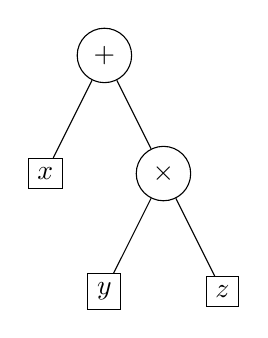
\begin{tikzpicture}
\node [circle,draw] {$+$}
  child {node [draw] {$x$}}
  child {
    node [circle,draw] (M) {$\times$}
    child {node [draw]{$y$}}
    child {node [draw]{$z$}}
  };
\end{tikzpicture}
\qquad\qquad
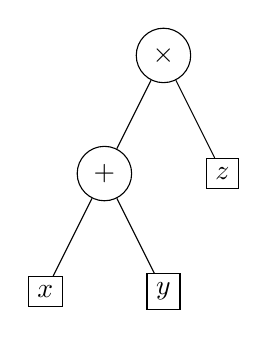
\begin{tikzpicture}
\node [circle,draw] {$\times$}
  child {
    node [circle,draw] (M) {$+$}
    child {node [draw]{$x$}}
    child {node [draw]{$y$}}
  }
  child {node [draw] {$z$}}
;
\end{tikzpicture}
\end{center}

Le regole di interpretazione della precedenza sono convenzionali
e possono esserci situazioni in cui non c'è una completa concordanza su come
una formula vada interpretata.
Quando le formule vengono rappresentate graficamente, inoltre,
anche la presentazione tipografica concorre nell'interpretazione
dell'ordine delle operazioni.
L'uso di spaziature, dimensioni e stili diversi oltre alla
posizione spaziale bidimensionale (linee di frazione, incolonnamenti)
intendono facilitare
l'interpretazione corretta dell'albero di valutazione riducendo
la necessità di utilizzare le parentesi.
\begin{comment}
Esempi di formule di dubbia interpretazione in
cui l'uso delle parentesi sarebbe invece auspicabile:
\[
  x/2\,y,\qquad
  \sin x \cdot 2, \qquad
  {e^x}^2, \qquad
  \frac{\displaystyle\frac{x}{y}}{z}.
\]
\end{comment}

\section{Calcolo dei predicati, quantificatori}

Possiamo pensare ai \myemph{predicati} come a proposizioni in cui
compaiono delle variabili.
Se una proposizione ha un valore di verità ben definito, il predicato
ha invece un valore di verità che dipende dal valore assegnato alle sue
variabili. Le variabili da cui dipende un predicato vengono chiamate
\myemph{variabili libere}. Le variabili libere possono venire \emph{chiuse}
(rese \emph{mute}) mediante operatori che agiscono
(estraendo un dato di sintesi) al variare della variabile su tutti i
suoi possibili valori.
Per quanto riguarda il calcolo proposizionale la chiusura delle variabili
di un predicato può essere fatta tramite i \myemph{quantificatori}
\emph{universale} $\forall$ (leggi: ``per ogni'') ed
\emph{esistenziale} $\exists$ (leggi: ``esiste'').
Ad esempio il predicato
$n>5 \Rightarrow n>m$ ha due variabili libere: $n$ ed $m$.
Possiamo chiudere la variabile $n$ con il quantificatore universale ottenendo:
\[
  \forall n \colon n>5 \Rightarrow n>m
\]
che è un predicato con una unica variabile libera $m$.
Il predicato può essere letto così: "per ogni $n$ se $n$ è maggiore di $5$ allora $n$ è anche maggiore di $m$."
Il valore di verità di questo
predicato dipende dal valore assegnato ad $m$.
Più precisamente il predicato è vero se $m\le 5$ ed è falso altrimenti.
La variabile $n$ è invece diventata muta, che significa che non ha più senso
assegnare dei valori alla variabile $n$ in quanto la verità di tale predicato non dipende più da $n$.

Per quanto riguarda l'intepretazione,
la proposizione ottenuta mediante un quantificatore universale
$\forall x\colon P(x)$ è vera se $P(x)$ è vera per ogni possibile valore
assegnato alla variabile $x$ ed è invece falsa se c'è anche un solo valore che
assegnato a $x$ rende falsa $P(x)$. Viceversa nella quantificazione
esistenziale $\exists x\colon P(x)$ si ottiene il vero nel caso ci sia almeno
un valore di $x$ che renda vera $P(x)$ e si ottiene il falso nel caso non ci sia
invece nessun valore di $x$ che renda vera $P(x)$.

Valgono in effetti le seguenti regole formali di scambio dei quantificatori con
la negazione logica:
\begin{align*}
  \neg \forall x \colon P(x) &\iff \exists x \colon \neg P(x)\\
  \neg \exists x \colon P(x) &\iff \forall x \colon \neg P(x).
\end{align*}
Osserviamo che queste relazioni corrispondono alle leggi di De Morgan per lo
scambio della negazione con gli operatori logici di congiunzione e disgiunzione.
Infatti l'operatore universale $\forall$ corrisponde ad una congiunzione logica
$\wedge$ su tutti i possibili valori del predicato,
così come l'operatore esistenziale
$\exists$ corrisponde ad una disgiunzione logica $\vee$.
Dal punto di vista mnemonico osserviamo che i simboli $\forall$ e $\exists$
si ottengono ruotando di 180 gradi le iniziali delle parole
\emph{All} ed \emph{Exists}.

Una variante dell'operatore esistenziale è l'operatore di unicità:
la proposizione $\exists! x\colon P(x)$ significa che esiste un \emph{unico} valore di $x$
che rende vero il predicato $P(x)$. Formalmente:
\[
  \exists!x\colon P(x) \iff \exists x\colon P(x)
  \wedge \neg \exists y\colon (y \neq x) \wedge P(y).
\]
Osserviamo che la precedente definizione utilizza il simbolo $\neq$ che è la
negazione dell'operatore di uguaglianza $=$ che verrà introdotto nella sezione
seguente.

\section{Teoria degli insiemi}

Fin'ora abbiamo presentato le regole logiche per la manipolazione dei valori di
verità dei predicati. Non abbiamo però ancora costruito nessun predicato né
tantomeno abbiamo introdotto gli oggetti che i predicati dovrebbero descrivere.

La teoria degli insiemi serve ad introdurre un \emph{universo} all'interno del
quale potremo identificare degli oggetti che possano rappresentare gli enti
matematici: numeri, funzioni, relazioni, insiemi.
Vedremo però che tutti questi enti matematici potranno essere ricondotti al
concetto di insieme: sarà dunque questo il concetto fondamentale che vogliamo
descrivere.

Quella che segue è la formalizzazione dovuta ai matematici Zermelo e Fraenkel.
Tale teoria viene comunemente chiamata $ZF$.

Intuitivamente gli \myemph{insiemi} sono collezioni di elementi.
Per costruire un sistema formale che descriva gli insiemi sarà sufficiente
introdurre un unico predicato che mette in relazione un elemento con l'insieme
che lo contiene:
\[
  x \in A
\]
(leggi: ``$x$ è un elemento di $A$``).
Indicheremo con $\not \in$ la negazione
di questa relazione.
Dovremo indicare quali sono le regole formali che ci permetteranno di manipolare
questo tipo di formule.
Sarà utile poter costruire insiemi di insiemi, quindi in realtà nel predicato precedente
$x$ potrebbe a sua volta essere un insieme. Dunque, per semplicità, supporremo
che tutti gli oggetti siano insiemi.

A partire dalla relazione di \myemph{appartenenza} $\in$ potremo definire le altre
relazioni tra insiemi:
\begin{align*}
  A \subset B &\iff \forall x\colon (x \in A \Rightarrow x \in B)\\
  A \supset B &\iff \forall x\colon (x \in A \Leftarrow x \in B)\\
  A = B & \iff A\subset B \,\wedge\, B\subset A.
\end{align*}

Il simbolo $\subset$ rappresenta l'\myemph{inclusione} tra insiemi.
Osserviamo che in altri testi potrà essere invece utilizzato il simbolo $\subseteq$
per rappresentare la stessa relazione
rendendo esplicito il fatto che non si esclude che i due insiemi siano
uguali (inclusione larga).

La terza delle regole precedenti si chiama \emph{assioma di estensionalità}
e definisce il fondamentale concetto di \myemph{uguaglianza}.
Il nostro sistema formale sarà dotato di opportune regole di inferenza che
garantiscano che se due oggetti sono uguali
potranno essere liberamente sostituiti uno con l'altro in qualunque
altra formula. Questo garantisce la proprietà transitiva dell'uguaglianza.
Si definirà la \myemph{disuguaglianza} $\not =$ come negazione dell'uguaglianza.

Vogliamo anche introdurre le usuali operazioni di \myemph{intersezione} $A\cap B$,
\myemph{unione}  $A\cup B$ e \myemph{differenza} $A \setminus B$
che possono essere codificate dai seguenti assiomi:
\begin{align*}
  x \in A \cap B &\iff (x \in A \wedge x \in B)\\
  x \in A \cup B &\iff (x \in A \vee x \in B)\\
  x \in A \setminus B &\iff x \in A \wedge x \not \in B.
\end{align*}

Più in generale possiamo richiedere di poter fare l'unione o l'intersezione
di una famiglia $\F$ non vuota di insiemi (una \emph{famiglia} di insiemi non è altro che un insieme di insiemi):
\begin{align*}
  x \in \bigcap \F &\iff \forall A \in \F\colon x \in A \\
  x \in \bigcup \F &\iff \exists A \in \F\colon x \in A.
\end{align*}
Spesso si usano le seguenti notazioni più espressive:
\[
 \bigcap \F = \bigcap_{A \in \F} A,\qquad
 \bigcup \F = \bigcup_{A \in \F} A.
\]

Per avere un primo oggetto su cui agire definiamo l'\myemph{insieme vuoto},
denotato
dal simbolo $\emptyset$, mediante il seguente assioma.

\begin{axiom}[insieme vuoto]
Esiste $\emptyset$ tale che
\[
\neg \exists x \colon x \in \emptyset.
\]
\end{axiom}

Osserviamo che le operazioni definite in precedenza, se applicate all'insieme vuoto,
non ci permettono di ottenere nuovi insiemi.
Per avere insiemi con un solo elemento introduciamo l'insieme \myemph{singoletto}
$\{ y \}$ cioè un insieme contenente un unico oggetto $y$:
\[
  x \in \{ y \} \iff x = y.
\]
A questo punto utilizzando l'unione possiamo già ottenere,
per elencazione,
insiemi con un numero
arbitrario (ma finito) di elementi, ad esempio:
\[
  \{a, b, c\} = \{ a \} \cup \{ b\} \cup \{c\}.
\]

Con le operazioni che abbiamo introdotto è già possibile descrivere infiniti insiemi
tra loro diversi. Ad esempio questi sono quattro insiemi diversi:
\[
 \emptyset,\quad
 \{ \emptyset \},\quad
 \{\{\emptyset\}, \emptyset\},\quad
 \{\{\emptyset\}, \{\{\emptyset\}\}\}
\]
mentre ognuno dei seguenti coincide con uno (quale?) dei precedenti:
\[
 \{\emptyset, \emptyset\},\quad
 \{\{\emptyset, \{\emptyset\}\}, \{\{\emptyset\}, \emptyset\}\}.
\]

Possiamo anche definire un insieme mediante una qualunque
proprietà che caratterizzi
i suoi elementi.

\begin{axiom}[specificazione]
Se $A$ è un insieme e $P(x)$ un predicato, allora
esiste un insieme $B$ denotato con $B = \{x\in A\colon P(x)\}$ tale
che si abbia:
\[
  b \in B \iff (b \in A) \wedge P(b).
\]
\end{axiom}

Osserviamo che viene richiesto a priori un insieme ambiente $A$ sul quale
viene ristretta la caratterizzazione. Questo significa che questo assioma non
può generare insiemi più grandi di quelli già esistenti.

Molte delle definizioni precedenti possono essere date mediante l'assioma
di specificazione. Ad esempio intersezione e differenza si possono
ricondurre all'unione:
\begin{align*}
  A \cap B &= \{x\in A \cup B \colon x\in A \land x \in B\},
  A \setminus B &= \{x\in A \colon x \not \in B\}.
\end{align*}


\section{Il paradosso di Russel}

La formalizzazione ZF che abbiamo esposto ha avuto una storia travagliata.
Nel 1902 Frege aveva tentato di assiomatizzare la teoria degli
insiemi introducendo l'assioma di specificazione nella forma seguente.

\begin{axiom}[specificazione ingenua]
  Se $P(x)$ è un predicato allora esiste un insieme
  $B$ denotato con $B=\{x\colon P(x)\}$ tale che
  \[
    x\in B \iff P(b).
  \]
\end{axiom}

Questo assioma è molto più potente di quello introdotto in precedenza perché
non vincola la specificazione agli elementi di un insieme già costruito.
In realtà Russel (ma prima ancora Zermelo) si accorse che tale assioma è talmente
potente da portare ad una contraddizione, che fa cadere
l'intera teoria ingenua degli insiemi (chiamiamo così la teoria degli insiemi
come era stata introdotta da Cantor e poi formalizzata da Frege).

\begin{paradox}[Russel]
Si consideri l'insieme (formalizzato in maniera ingenua)
\[
  R = \{ x\colon x \not\in x\}.
\]
Allora $R\in R \iff R\not \in R$. Assurdo.
\end{paradox}

Il paradosso di Russel può essere espresso anche nella lingua naturale.
Una delle sue accezioni più note si chiama \emph{Paradosso del barbiere}
e si enuncia come segue. Il \emph{barbiere} è quella persona che fa la barba
alle persone che non se la fanno da se. Il barbiere si fa la barba da se?

Un'altro modo di esprimere il paradosso di Russel nel linguaggio naturale
riguarda l'utilizzo degli aggettivi ed è il seguente. Diremo che un aggettivo
è \emph{autologico} se esso stesso soddisfa la proprietà che descrive.
Ad esempio l'aggettivo \emph{polisillabico} è polisillabico e dunque è
autologico. Lo stesso vale per l'aggettivo \emph{sdrucciolo}
che è autologico in quanto è una parola con l'accento sulla terz'ultima sillaba.
Gli aggettivi che non sono autologici li chiameremo \emph{eterologici}.
Ci si può allora chiedere se l'aggettivo \emph{eterologico} è eterologico.
Anche in questo caso si arriverà ad un paradosso perché se \emph{eterologico}
fosse eterologico allora sarebbe autologico cioè non eterologico.
Viceversa se eterologico fosse autologico allora sarebbe eterologico cioè
non autologico.

Il paradosso di Russel non si applica alla teoria ZF che abbiamo introdotto
in quanto in tale teoria l'assioma di specificazione richiede un insieme
ambiente in cui il predicato viene valutato.
Se fissiamo un insieme \emph{ambiente} $U$ poossiamo definire il seguente:
\[
  R = \{ x \in U \colon x \not \in x\}.
\]
In tal caso abbiamo che $R\in R$ se e solo se $(R\in U) \land (R \not \in R)$.
In particolare se fosse $R\in R$ avremmo un assurdo. Ma non è invece
assurdo che $R\not \in R$, infatti in tal caso potrà essere (anzi, dovrà essere)
$R\not \in U$.
Non abbiamo ottenuto un paradosso, ma abbiamo scoperto che dato
un qualunque insieme $U$ esiste un insieme $R$ che non sta in $U$.
Questo significa che non esiste l'insieme \myemph{universo}, cioè un insieme che
contiene tutti gli insiemi. Osserviamo che l'insieme universo sarebbe il complementare
dell'insieme vuoto, e questo è il motivo per cui non è possibile definire
il complementare di un insieme ma ci si limita a definire la differenza tra insiemi.

La relazione $x\in x$ potrebbe di per se sembrare contraddittoria.
Come è possibile che un insieme contenga se stesso come elemento?
Se ad esempio avessimo $x=\{ x\}$ si avrebbe $x=\{\{x\}\} = \{\{\{ x\}\}\} \dots$
e così via in una discesa infinita che non avrebbe mai termine.
La possibilità che esistano insiemi di questo tipo è piuttosto fastidiosa ed è per questo
che si pone l'assioma di \emph{fondazione} (o di \emph{regolarità}) che afferma
in particolare che non esistono insiemi $x$ tali che $x\in x$.
Più in generale l'assioma di fondazione evita che sia possibile
costruire una catena discendente infinita di insiemi che siano
elemento uno dell'altro:
\[
  \dots \in x_n \in \dots \in x_2 \in x_1.
\]
Osserviamo però che anche assumendo che $x\not\in x$ sia sempre vera,
il paradosso di Russel rimane valido, in tal caso infatti
$R=\{x\colon x\not \in x\}$ dovrebbe contenere
tutti gli insiemi e quindi dovrebbe essere $R\in R$... che abbiamo escluso.

Un altro modo per dimostrare che è sempre possibile costruire un
insieme \emph{più grande} di un insieme dato si ottiene dall'insieme potenza
(che vediamo subito) tramite il teorema di Cantor (che vedremo più avanti).

L'assioma dell'insieme potenza, serve
a garantire l'esistenza del\-l'\myemph{insieme delle parti}.
Se $X$ è un qualunque insieme si può considerare $\P(X)$ come l'insieme dei
sottoinsiemi di $X$:
\[
 A \in \P(X) \iff A \subset X.
\]
L'insieme $\P(X)$ si chiama anche \emph{insieme potenza} e viene a volte indicato con $2^X$
in quanto se $X$ ha $n$ elementi allora $\P(X)$ ha $2^n$ elementi.
Ad esempio se $X=\{a, b, c\}$ ha tre elementi, l'insieme delle parti
ha otto elementi:
\[
 \P(X) = \{ \{\}, \{a\}, \{b\}, \{c\}, \{a,b\},
   \{a,c\}, \{b,c\}, \{a,b,c\}\}.
\]
Inteso che $\{\}=\emptyset$ osserviamo che l'insieme vuoto è sottoinsieme di
qualunque altro insieme (verificarlo tramite la definizione),
dunque appartiene sempre all'insieme delle parti.
L'insieme delle parti risulta fondamentale per poter esprimere
la \emph{logica del secondo ordine} ovvero la possibilità di poter
formulare predicati sui sottoinsiemi di un insieme invece che solamente
sui suoi elementi.

\section{Relazioni e funzioni}

Definiamo la \myemph{coppia ordinata} $(a,b)$ come un oggetto (un insieme,
visto che abbiamo deciso che tutti gli oggetti matematici sono insiemi) con
la seguente proprietà:
\begin{equation}\label{def:pair}
  (a,b) = (c,d) \iff a=c\, \wedge \,b=d.
\end{equation}
In particolare $(a,b) \neq (b,a)$ se $a\neq b$ cioè l'ordine dei due elementi
è importante.
Formalmente si potrebbe definire $(a,b)=\{\{a\}, \{a,b\}\}$,
si provi per esercizio a dimostrare che con questa definizione vale la
proprietà~\eqref{def:pair}.
Se $A$ e $B$ sono insiemi dati, l'insieme di tutte le coppie di elementi
presi il primo da $A$ e il secondo da $B$ si indica con $A \times B$ e si chiama
\myemph{prodotto cartesiano}:
\[
x \in A \times B \iff \exists a \in A, \exists b \in B\colon x = (a,b).
\]
Se $A$ ha $n$ elementi e $B$ ha $m$ elementi, il prodotto $A\times B$ ha $n\cdot m$
elementi. Ad esempio se $A=\{a,b,c\}$ ha tre elementi e $B=\{a,b\}$ ha due elementi,
il prodotto ha sei elementi:
\[
  A \times B = \{(a,a), (a,b), (b,a), (b,b), (c,a), (c,b)\}.
\]

Una \myemph{relazione} $R$ tra gli elementi di un insieme $A$
e gli elementi di un insieme $B$
non è altro che un sottoinsieme del prodotto cartesiano: $R\subset A \times B$.
Scriveremo $x R y$ quando $(x,y) \in R$.
Ad esempio su un insieme di numeri potremmo considerare come $R$ la relazione d'ordine
$\le$ per cui scriveremo $x \le y$ quando $(x,y)\in R$.
Le relazioni da un insieme in sé stesso possono eventualmente avere particolari caratteristiche
come essere: \emph{transitive} ($xRy \wedge yR z \implies x R z$),
\emph{simmetriche} ($xRy \implies yRx$),
\emph{riflessive} ($xRx$).
Come esercizio si provi a pensare alla relazione tra persone $xAy$
definita dalla frase "$x$ ama $y$".
Si consideri il significato delle proprietà transitiva, simmetrica
e riflessiva di tale relazione.

Possiamo pensare ad una coppia $(a,b)$ come ad una freccia che
parte da $a$ e arriva in $b$: $a \mapsto b$.
Potremmo scrivere più espressivamente $(a,b)\in R$ come
$a \stackrel{R}\mapsto b$.
In questo modo una relazione su $A\times B$
risulta essere un insieme di frecce che partono da elementi di $A$
ed arrivano su elementi di $B$. La rappresentazione che si ottiene prende
anche il nome di \emph{grafo orientato}.
Si provi ad interpretare \emph{graficamente} le proprietà
transitiva, simmetrica e riflessiva di un grafo.

Ogni relazione può essere \emph{invertita}\marginpar{relazione inversa}
semplicemente scambiando il ruolo
dei due insiemi $A$ e $B$. Se $R$ è una relazione e vale $x R y$
per la relazione inversa $R'$ si avrà
$y R' x$.
Pensando ad una relazione $R$ come un insieme di frecce
$x\stackrel R \mapsto y$,
la relazione inversa $R'$ risulta essere lo stesso insieme di frecce ma
con la direzione opposta $y\stackrel{R'} \mapsto x$.

Le relazioni che più ci interesseranno in questo corso sono le \myemph{funzioni}.
Le funzioni sono le relazioni \emph{univoche} cioè quelle relazioni $f$ in
$A\times B$ che
mandando (nel senso delle frecce) ogni elemento $a\in A$ in uno
ed un solo elemento
$b\in B$:
\[
\forall a\in A\colon \exists ! b\in B\colon a\stackrel{f}\mapsto b.
\]
Tale unico elemento $b\in B$ associato all'elemento $a\in A$ viene chiamato
\emph{immagine} di $a$ tramite $f$ e viene indicato con $b=f(a)$.
Una funzione definita da $A$ in $B$ si indica con $f\colon A \to B$. L'insieme
$A$ viene chiamato \myemph{dominio} e l'insieme $B$ \myemph{codominio}.

Le funzioni vengono spesso utilizzate per rappresentare delle trasformazioni.
Possiamo pensare ad una funzione come ad una scatola nera (un macinino)
a cui possiamo dare in pasto elementi dell'insieme $A$ (\emph{input})
e otteniamo come risposta elementi dell'insieme $B$ (\emph{output}).

Se l'output (codominio) di una funzione $f$
coincide con l'input (dominio) di una funzione $g$,
cioè se $f\colon A \to B$ e $g\colon B \to C$
possiamo comporre\marginpar{funzione composta}
le due funzioni per ottenere una funzione
$g\circ f \colon A \to C$:
\[
(g\circ f)(x) = g(f(x))\qquad
x \stackrel f \mapsto f(x) \stackrel g \mapsto g(f(x)).
\]

Vedremo come la composizione ci permette di costruire innumerevoli funzioni
componendo tra loro poche funzioni elementari, così come si può costruire un edificio
utilizzando semplici mattoni.
Ovviamente sarà importante conoscere a fondo
tutte le caratteristiche dei mattoni (proprietà delle funzioni elementari)
e sarà pure importante capire come tali proprietà si combinano quando mettiamo
insieme i diversi blocchi.

Uno dei problemi più importanti a
cui si può probabilmente ricondurre qualunque problema
matematico è quello dell'invertibilità di una funzione: data $f\colon A\to B$
trovare una funzione $g\colon B\to A$ tale che
se $x\stackrel f \mapsto y$ allora
$y \stackrel g\mapsto x$. Se ad esempio io so qual è la traiettoria di
un proiettile in funzione dell'angolo di tiro, mi chiedo quale angolo devo
scegliere per centrare un determinato bersaglio.
Oppure (altro esempio) data la funzione $f(x) = x^2$ (definita su un qualche insieme
numerico) dire se è possibile trovare $x$ tale che $f(x) = 2$
(definizione della radice quadrata).
Oppure ancora: se $x A y$ è la relazione ``$x$ ama $y$''
e se io sono $y$ sarei interessato a trovare gli $x$ tali che $x A y$.

Per poter invertire una funzione $f\colon A \to B$ abbiamo la necessità di verificare due
differenti proprietà: che per ogni $b\in B$ esista un elemento $a\in A$ tale che $f(a)=b$
(surgettività)
e che tale elemento $a$ sia unico (iniettività).
Più precisamente diremo che $f\colon A\to B$ è \myemph{surgettiva} se
\[
  \forall b\in B\colon \exists a \in A \colon f(a) = b
\]
ed è \myemph{iniettiva} se
\[
 \forall a\in A, \forall a'\in A\colon (f(a) = f(a') \implies a=a').
\]
Se una funzione $f\colon A \to B$ è iniettiva e surgettiva allora
si dice che $f$ è \myemph{bigettiva} o \myemph{invertibile}.
La funzione $g\colon B \to A$ che ad ogni
$b\in B$ associa l'unico $a\in A$ tale che $f(a)=b$ si chiama
\emph{funzione inversa} di $f$.
Tale funzione $g$ si indica anche con il simbolo $f^{-1}$ ed ha le proprietà
\[
  \forall x \in A\colon g(f(x)) = x, \qquad
  \forall y\in B\colon f(g(y)).
\]
La funzione inversa di $f$ è quindi anch'essa invertibile e l'inversa dell'inversa
è $f$ stessa: $(f^{-1})^{-1} = g^{-1} = f$.

L'insieme di tutte le funzioni $f\colon A \to B$ viene denotato con $B^A$.
L'insieme di tutte le funzioni $f\colon A \to A$ potrà essere
denotato con $A!$ o (più comunemente) con $S(A)$
(si veda l'esercizio~\ref{ex:9478} per avere una motivazione di tali notazioni).



Se $f\colon X\to Y$ è una funzione e se $A\subset X$ si definisce
l'insieme $f(A)$, chiamato \myemph{immagine} di $A$ tramite $f$ come:
\[
  f(A) = \{f(x)\colon x \in A\}
\]
se invece $B\subset Y$ si definisce l'insieme $f^{-1}(B)$, chiamato
\myemph{controimmagine} di $B$ tramite $f$ come:
\[
  f(B) = \{x\in A \colon f(x) \in B\}.
\]
Notiamo innanzitutto che la prima definizione non rientra esattamente
nell'assioma di specificazione ma è un modo più immediato per intendere
la seguente definizione che è invece perfettamente valida:
\[
  f(A) = \{y\in B \colon \exists x\in A \colon f(x) = y\}.
\]
Notiamo inoltre che questa definizione rappresenta un \emph{abuso di notazione}.
Infatti avevamo già dato una definizione per il simbolo $f(x)$.
Questa notazione va quindi utilizzata solo se il contesto rende chiaro il fatto
che $A$ va inteso come un sottoinsieme del dominio di $f$ e non come un elemento
di tale dominio.

Se $A=X$ è l'intero dominio della funzione
l'insieme $f(X)$ si chiama \emph{immagine di $f$}.
Possiamo allora osservare che una funzione $f\colon X \to Y$ risulta essere
surgettiva se e solo se $f(X) = Y$.
Se prendiamo un qualunque $y\in Y$ possiamo considerare l'insieme $f^{-1}(\{y\})$
che è sempre definito, anche se $f$ non fosse invertibile. Se tale insieme ha sempre
almeno un elemento significa che la funzione è surgettiva. Se tale insieme ha
sempre non più di un elemento significa che la funzione è iniettiva.
Se tale insieme ha sempre esattamente un elemento allora la funzione è invertibile
e si ha $f^{-1}(\{y\}) = \{f^{-1}(y)\}$.

Questo abuso di notazione
(inserire un insieme dove dovrebbe starci un singolo elemento)
potrà essere utilizzato anche con gli operatori infissi.
Una operazione, rappresentata ad esempio dal simbolo $+$, può essere pensata
come ad una funzione che agisce su una coppia di valori: $+\colon X\times Y \to Z$.
La notazione $x+y$ serve quindi ad abbreviare la notazione $+(x,y)$.
Anche in questo caso potrà capitare che al posto di $x$ o di $y$ o di entrambi,
si inserisca un insieme di valori:
\begin{align*}
   A + y &= \{x+y\colon x \in A\}, \\
   x + B &= \{x+y\colon y \in B\}, \\
   A + B &= \{x+y\colon x\in A, y \in B\}.
\end{align*}
In tutti questi casi il risultato è un insieme di valori, invece che un singolo
valore.

In maniera simile, questo abuso viene attuato anche con le relazioni.
Se ad esempio abbiamo
una relazione $x\le y$, e $A, B$ sono insiemi, si potrà intendere
che valgano le seguenti notazioni:
\begin{align*}
  x \le B &\iff (\forall y\in B\colon x\le y), \\
  A \le y &\iff (\forall x\in A\colon x \le y), \\
  A \le B &\iff (\forall x\in A, \forall y\in B\colon x\le y).
\end{align*}

\begin{exercise}
Se $R$ è una relazione tra $A$ e $B$ si dia una definizione di $R(C)\subset B$
quando $C\subset A$ in modo che tale definizione coincida con la definizione
di \emph{immagine} se $R$ è una funzione.
Si osservi che con tale definizione la controimmagine di un insieme tramite
una funzione $f$ non è altro che l'immagine tramite la relazione inversa $f^{-1}$
(ricordando che ogni funzione essendo una relazione ha una relazione inversa).
\end{exercise}

\section{I numeri naturali}

\begin{theorem}[assiomi di Peano]
  L'insieme $\NN$ dei numeri naturali è un insieme su cui
  è data una funzione $\sigma\colon \NN\to\NN$ e un
  elemento $0\in \NN$ (chiamato \myemph{zero}) che soddisfano le seguenti proprietà.
  \begin{enumerate}
  \item $\sigma$ è iniettiva;
  \item non esiste $n\in \NN$ tale che $\sigma(n)=0$;
  \item (assioma di induzione)
  \index{assioma!di induzione}
  per ogni $A\subset \NN$ se
  \begin{enumerate}
     \item $0\in A$;
     \item $\forall n\in \NN \colon n\in A \implies \sigma(n) \in A$;
  \end{enumerate}
  allora $A= \NN$.
  \end{enumerate}
\end{theorem}

I numeri naturali sono i numeri utilizzati per \emph{contare}.
La funzione $\sigma\colon \NN \to \NN$ rappresenta il successore di un numero
naturale, quindi quando avremo definito la somma vedremo che sarà
$\sigma(n)=n+1$.
Il fatto che $\sigma$ sia iniettiva serve a esprimere il fatto che
durante un conteggio non si torna mai ad un numero già utilizzato.
Lo zero è inoltre particolare perché esso non è il successore di nessun altro
numero naturale (questo viene espresso dal secondo assioma).
L'ultimo assioma serve a garantire che partendo da zero e cominciando
a considerare il suo successore (che si chiama $1=\sigma(0)$) e poi il
successore del successore (chiamato $2=\sigma(1)$) e così via, si ottengono
tutti i numeri naturali. Vedremo, ad esempio, che l'insieme $\QQ^+$
dei numeri razionali non negativi
soddisfa i primi due assiomi di Peano se si pone $\sigma(q)=q+1$
ma non soddisfa il terzo assioma in quanto la frazione $1/2$ non viene mai raggiunta
partendo da $0$ e sommando $1$.

L'esistenza di un insieme che soddisfa gli assiomi di Peano non è garantita
dagli assiomi visti finora. Sarà necessario un assioma apposito.
Tale assioma si chiama \emph{assioma di infinito} in quanto, come vedremo
nel Teorema~\ref{th:4994}, è equivalente a supporre l'esistenza di un
qualunque insieme infinito.

\begin{axiom}[di infinito]
  Esiste un insieme $\NN$ che soddisfa gli assiomi di Peano.
\end{axiom}

La proprietà induttiva dei numeri naturali permette di definire le funzioni su
$\NN$ utilizzando le \emph{definizioni per induzione}, come nel seguente.
%
\begin{theorem}[definizione per induzione]\label{th:def_induction}
Sia $A$ un insieme, $\alpha \in A$ e $g\colon \NN\times A \to A$.
Allora esiste un unica funzione $f\colon \NN \to A$ tale che
\begin{equation}\label{eq:485452}
\begin{cases}
  f(0) = \alpha,\\
  \forall n\in \NN\colon f(\sigma(n)) = g(n, f(n)).
\end{cases}
\end{equation}
(La parentesi graffa serve ad indicare che entrambe le condizioni devono
essere soddisfatte contemporaneamente).
\end{theorem}
%
Intuitivamente dopo aver definito $f(0) = \alpha$ si potrà definire
$f(1) = g(0, \alpha)$, $f(2) = g(1, f(1))$, $f(3) = g(2, f(2))$ etc.
Per la proprietà induttiva dei numeri naturali la funzione $f$ risulterà
definita univocamente su tutti i numeri naturali.
Riportiamo di seguito una dimostrazione più formale, che ci permette di
osservare come viene utilizzata in pratica la definizione di funzione.
%
\begin{proof}
L'idea della dimostrazione è di definire $f$ come la ``più piccola'' relazione
che soddisfa le condizioni~\eqref{eq:485452}. Si prenderà poi l'insieme su cui $f$
è definita univocamente e si dimostrerà che è tutto $\NN$ concludendo quindi
che è una funzione $f\colon \NN \to A$.

Consideriamo l'insieme di tutte le relazioni tra $N$ e $A$
che soddisfano~\eqref{eq:485452}:
\begin{align*}
\mathcal F = \{ R\subset \NN \times A \colon &(0,\alpha)\in R,\\
  &(n,a)\in R \implies (\sigma(n),g(n,a))\in R \}
\end{align*}
e definiamo
\[
  f = \bigcap \mathcal F.
\]
Chiaramente $f\subset \NN\times A$ è una relazione.
E' anche facile verificare che $f\in \mathcal F$ (si ragioni sulla
definizione di intersezione).
Posto
\[
  D = \{ n\in \NN\colon \exists! a\in A\colon (n,a)\in f \}
\]
vogliamo dimostrare che $D=\NN$.
Lo possiamo fare utilizzando l'assioma di induzione.
Visto che $f\in \mathcal F$ sappiamo che $(0,\alpha)\in f$.
Se esistesse $a\neq \alpha$ tale che $(0,a)\in f$ allora potrei considerare la
relazione $R = f \setminus \{(0,a)\}$ e osservare che $R\in \mathcal F$
(visto che $a\neq \alpha$ questo non inficia la condizione $(0,\alpha)\in R$ e
visto che $\sigma(n)\neq 0$ non viene inficiata neanche la condizione
$(n,a)\in R \implies (\sigma(n),g(n,a))\in R$.
Siccome $R\in \mathcal F$
e $R\subset f$ otteniamo una contraddizione in quanto essendo $f=\bigcap \mathcal F$
si dovrebbe avere $f\subset R$ e quindi $f=R$, cosa che non è.
Abbiamo quindi mostrato che $0\in D$ che è la prima condizione nell'assioma di induzione.

Supponiamo ora di sapere che $n\in D$: dobbiamo allora dimostrare che anche
$\sigma(n)\in D$. Ma se $n\in D$ significa che esiste un unico $a\in A$ tale che
$(n,a)\in f$. Essendo $f\in \mathcal F$ questo implica che $(\sigma(n),g(n,a))\in R$
e quindi esiste $b=g(n,a)$ tale che $(\sigma(n),b)\in R$. Dobbiamo mostrare
che tale $y$ è unico. Se ci fosse $c\neq b$ tale che $(\sigma(n),c)\in f$ potrei
definire (analogamente a come abbiamo fatto nel passo precedente)
$R=f\setminus\{(\sigma(n),c)\}$. Anche in questo caso possiamo dimostrare
che $R\in \mathcal F$.
Certamente $(0,\alpha)\in f$ ed essendo $\sigma(n)\neq 0$ possiamo
affermare che $(0,\alpha)\in R$.
Inoltre se $(k,d)\in R$ allora certamente $(k,d)\in f$ (in quanto $R\subset f$)
e quindi $(\sigma(k),g(k,d))\in f$ dunque basta escludere che sia
$(\sigma(k),g(k,d)) = (\sigma(n),c)$.
Questo succede in quanto se fosse $\sigma(k)=\sigma(n)$ avremmo $k=n$
e quindi $d=a$ in quanto $n\in D$. Ma allora si avrebbe $g(k,d)=g(n,a)=b\neq c$.

L'assioma di induzione può dunque essere applicato e ci permette di concludere
che $D=\NN$. Significa che $f$ è univocamente definita su tutto $\NN$ e quindi
è una funzione $f\colon \NN \to A$ che soddisfa~\eqref{eq:485452} in
quanto $f\in \mathcal F$.
\end{proof}

Con questo tipo di definizioni è possibile definire per induzione
l'operazione $+$ (addizione)
facendo in modo che valga la seguente proprietà:
\[
\begin{cases}
  n + 0 = n\\
  n + \sigma(m) = \sigma(n+m).
\end{cases}
\]
In particolare si ottiene $\sigma(n) = n+1$ e quindi d'ora in avanti
non useremo più la funzione $\sigma$ ma useremo sempre l'addizione.
Analogamente sarà
 possibile definire la moltiplicazione $\cdot$ in modo che
valga
\[
\begin{cases}
  n\cdot 0 = 0 \\
  n \cdot \sigma(m) = n\cdot m + n.
\end{cases}
\]
Si potrà poi verificare (cosa elementare ma non semplice)
che le operazioni così definite soddisfano le ben
note proprietà:
\begin{enumerate}
\item $n+0=n$, $n\cdot 1 = n$ (esistenza degli elementi neutri);
\item $n+m = m+n$, $n\cdot m = m\cdot n$ (proprietà commutativa);
\item $n\cdot (a+b) = n\cdot a + n\cdot b$ (proprietà associativa).
\end{enumerate}

% Diremo che un numero $n\in \NN$ è divisibile per $m\in \NN$ se esiste $k\in \NN$
% tale che $n = k \cdot m$. In tal caso scriveremo $k = n/m$.

Si potrà anche definire una relazione d'ordine $\le$ tramite la condizione
\[
  n \le m \iff \exists k \in \NN \colon m = n+k.
\]
La relazione $\ge$ si definisce come la relazione inversa di $\le$.
La relazione $<$ si
definisce richiedendo che sia $x\le y \land x\neq y$ e la relazione $>$
è definita come l'inversa di $<$.

Come esempio di applicazione della definizione per induzione definiamo
il \emph{fattoriale} $n! = 1 \cdot 2 \dots n$ (il prodotto dei numeri naturali
da $1$ a $n$).
Per definire tale funzione
$\NN \to \NN$ in maniera rigorosa osserviamo che il prodotto dei numeri da $1$
a $n+1$ può essere definito come il prodotto dei numeri da $1$ a $n$ moltiplicato
per $n+1$. Imponendo poi che\footnote{%
E' chiaro che deve essere $1!=1$ e di conseguenza se vale $(n+1)! = (n+1)\cdot n!$
dovrà essere $0!=1$.
D'altra parte è naturale che il prodotto di un insieme vuoto di numeri sia
l'elemento neutro del prodotto, così come la somma di zero numeri è l'elemento
neutro della somma.
}
$0!=1$, si ottiene una caratterizzazione univoca:
\[
 \begin{cases}
  0! = 1 \\
  (n+1)! = (n+1) \cdot n!
 \end{cases}
\]
Si tratta di applicare il Teorema~\ref{th:def_induction}
con $A=\NN$, $\alpha = 1$, $g(n, a) = (n+1)\cdot a$ per garantire che esiste
una unica funzione $\NN\to\NN$, $n\mapsto n!$, che soddisfa queste proprietà.

In maniera simile si potrà definire per ogni $n,m \in \NN$ l'elevamento a potenza $n^m$
in modo che valga\footnote{%
Si noti che stiamo definendo $0^0=1$.
Alcuni testi lasciano indefinita questa operazione ma in realtà la formula
è giustificata dal fatto che $0^0$ è un prodotto di $0$ fattori e quindi,
come $0!$, deve valere $1$.
Questo viene confermato dal fatto che $n^m$ è il numero di funzioni da un
insieme con $m$ elementi in un insieme con $n$ elementi e
su un dominio vuoto è definita una unica funzione (la funzione vuota)
qualunque sia il codomonio.
}
\[
\begin{cases}
  n^0 = 1\\
  n^{m+1} = n\cdot n^m.
\end{cases}
\]

La proprietà induttiva dei numeri naturali è equivalente al seguente.
\begin{theorem}[principio di induzione]
Sia $P(n)$ un predicato sui numeri naturali $n\in \NN$.
Se valgono le seguenti condizioni
\begin{enumerate}
\item $P(0)$ è vera
\item $P(n) \implies P(n+1)$
\end{enumerate}
allora $P(n)$ è vera per ogni $n\in \NN$.
\end{theorem}
%
\begin{proof}
Si consideri l'insieme $A=\{n\in \NN\colon \text{$P(n)$ è vera}\}$ e si
applichi il terzo assioma di Peano per verificare che $A=\NN$.
\end{proof}


\begin{exercise}
La somma $S(n) = 1 + 2 + \dots +n$
dei naturali da $1$ fino a $n$ può essere definita come quella unica funzione
che soddisfa le proprietà
\[
\begin{cases}
  S(0) = 0 \\
  S(n+1) = S(n) + (n+1).
\end{cases}
\]
Dimostrare che $S(n) = n \cdot (n+1) / 2$.
\end{exercise}

\begin{exercise}
Dimostrare che per la somma
$Q(n) = 1^2 + 2^2 + \dots + n^2$
(somma dei quadrati dei naturali da $1$ a $n$)
vale la formula
$Q(n) = n \cdot (n+1)\cdot (2n + 1) / 6$.
\end{exercise}

Potrà risultare utile utilizzare le seguenti varianti del principio di
induzione
\begin{theorem}[principio di induzione (variante)]
Sia $P(n)$ un predicato definito sui numeri naturali $n$
non inferiori a $n_0\in \NN$.
Se
\begin{enumerate}
\item $P(n_0)$ è vero
\item $P(n) \implies P(n+1)$ per ogni $n\ge n_0$
\end{enumerate}
allora $P(n)$ è vero per ogni $n\ge n_0$.
\end{theorem}

\begin{theorem}[principio di induzione forte]
Sia $P(n)$ un predicato definito sui numeri naturali $n\in \NN$.
Se
\begin{enumerate}
\item $P(0)$ è vero
\item $(\forall k\le n\colon P(k))\implies P(n+1)$
\end{enumerate}
Allora $P(n)$ è vero per ogni $n\in \NN$.
\end{theorem}

\begin{definition}[massimo/minimo]
  Se $\le$ è una relazione d'ordine definita su un insieme $X$ e
  $A\subset X$ diremo che $a$ è un \emph{massimo} di $A$ e
  scriveremo
  \[
    a = \max A
  \]
  se $a\in A$ e $A\le a$ (cioè $x\le a$ per ogni $x\in A$).
  Diremo che $a$ è un \emph{minimo} di $A$ e scriveremo
  \[
    a = \min A
  \]
  se $a\in A$ e $a\le A$ (cioè $a\le x$ per ogni $x\in A$).
\end{definition}

E' facile dimostrare che se prendiamo $I_n = \{k\in \NN\colon k<n\}$
ogni sottoinsieme non vuoto $A$ di $I_n$ ha sia massimo che minimo
(lo si dimostri per induzione su $n$). Su tutto $\NN$ esistono
però degli insiemi non vuoti che non hanno massimo. Ad esempio l'insieme
dei numeri pari:
$2\cdot \NN = \{2k\colon k\in \NN\}$ non ha massimo perchè se $n$ è pari
anche $n+2$ è pari ed è strettamente maggiore di $n$.

\begin{theorem}[buon ordinamento di $\NN$]
Se $A$ è un sottoinsieme non vuoto di $\NN$ allora
$A$ ha minimo.
\end{theorem}
%
\begin{proof}
Supponiamo per assurdo che $A$ non abbia minimo e consideriamo l'insieme
$B=\{b\in \NN\colon b \le A\}$.
Chiaramente $0\in B$ in quanto $0\le \NN$. Se poi sapessimo che $n\in B$
allora $n\le A$. Non può essere $n\in A$ altrimenti $n$ sarebbe il minimo di $A$.
Dunque $n < A$ e quindi $n+1 \le A$. Abbiamo quindi mostrato che se $n\in B$ anche $n+1\in B$.
Per il principio di induzione deduciamo che $B=\NN$ e quindi $A$ sarebbe vuoto,
cosa che abbiamo escluso per ipotesi.
\end{proof}


\section{Il teorema di incompletezza di G\"odel (cenni)}

Il teorema di incompletezza di G\"odel afferma che ogni
sistema formale sufficientemente potente (diciamo che sia in grado di
descrivere i numeri naturali come abbiamo fatto noi) è incompleto.
La dimostrazione di tale risultato rivoluzionario richiederebbe un intero
corso di logica, ma possiamo solo accennare al fatto che l'idea della
dimostrazione consiste nell'associare un numero naturale ad ogni formula
del sistema, tradurre tutte le regole di inferenza in operazioni aritmetiche
in modo tale da poter formalizzare le dimostrazioni all'interno del sistema
stesso. Dopodiché ``basterà'' trovare un numero $G$ tale per cui
l'enunciato corrispondente a $G$ significa:
"l'enunciato corrispondente al numero $G$ non può essere dimostrato",
ovvero: "\emph{questo} enunciato non può essere dimostrato".
E' chiara l'analogia con il paradosso di Epimenide: "questa frase è falsa".

Si osservi che l'enunciato $G$ di G\"odel non parla direttamente di verità,
che è un concetto esterno al sistema formale
(dipende dal modello che noi diamo al sistema).
Ma se vogliamo attaccare un valore di verità ad ogni enunciato dovremo decidere
se $G$ è vero o falso. Se è vero avremmo un sistema in cui un enunciato vero
non può essere dimostrato e quindi tale sistema sarebbe incompleto.
Se invece $G$ è falso avremmo un sistema in cui un enunciato falso può essere
dimostrato e quindi tale sistema sarebbe \myemph{incoerente} (ci sono degli assiomi
falsi oppure delle regole di inferenza che permettono di dedurre enunciati falsi
a partire da enunciati veri).

\section{Cardinalità}

La teoria degli insiemi è nata con l'intento di formalizzare l'utilizzo degli
insiemi con infiniti elementi. Infatti finché gli insiemi hanno un numero finito
di elementi non ci sono dubbi sulle loro proprietà. L'utilizzo di insiemi con
infiniti elementi, invece, ci pone di fronte a questioni che possono sembrare
paradossali.

Per confrontare gli insiemi finiti è sufficiente contare il numero degli elementi.
Diremo che un insieme è \emph{più grande} se ha un numero di elementi maggiore.
Ma se gli insiemi sono infiniti, non siamo in grado di effettuare un conteggio
degli elementi. Possiamo però osservare che non è necessario contare il numero
di elementi per poter dire che due insiemi hanno la stessa numerosità.
Ad esempio in un parcheggio pieno posso dire che il numero di automobili
è uguale al numero di posti, senza dover contare né l'uno né l'altro ma semplicemente
osservando che c'è una corrispondenza biunivoca tra i posti e le auto. Faremo
lo stesso per confrontare insiemi infiniti.

Diciamo che due insiemi $A$ e $B$ sono equipotenti e scriveremo $\#A = \#B$
se esiste una funzione bigettiva $f\colon A \to B$.
Il simbolo $\#A$ si chiama \myemph{cardinalità} di $A$ e quindi due insiemi
sono equipotenti se hanno la stessa cardinalità.
In tal caso la funzione
$f$ è invertibile e l'inversa è anch'essa bigettiva,
quindi se $\#A = \#B$ risulta anche $\#B = \#A$.
Tramite la composizione è inoltre facile verificare che se $\#A = \#B$ e $\#B = \#C$
allora $\#A = \#C$.
Nel caso degli insiemi finiti vedremo che la cardinalità coincide con il
numero di elementi dell'insieme, ma ci potranno essere anche cardinalità
\emph{infinite}.

La relazione di equipotenza definisce il concetto di cardinalità, specificando
quali sono gli insiemi che hanno la stessa cardinalità. Possiamo anche mettere
un ordinamento tra gli insiemi, specificando che un insieme $A$ ha cardinalità
minore o uguale a quella di $B$, $\#A\le \#B$, se esiste una funzione
iniettiva $f\colon A \to B$. Scriveremo $\#A < \#B$ per indicare che
$\#A \le \#B$ ma non $\#A = \#B$ (dunque esistono funzioni iniettive da $A$ in $B$
ma nessuna di queste risulta essere surgettiva).

Non è difficile verificare che se esiste una funzione iniettiva $f\colon A\to B$
allora esiste anche una funzione surgettiva $g\colon B\to A$
(basta osservare che una funzione iniettiva $f$ è invertibile sulla propria
immagine $f\colon A \to f(A)$ e la funzione inversa può essere estesa a
tutto $B$ in maniera arbitraria).
Più delicato mostrare il viceversa cioè che se esiste una funzione surgettiva
$g\colon B \to A$ allora esiste una funzione iniettiva $f\colon A \to B$.
Intuitivamente si tratta di scegliere, per ogni elemento $b\in B$, un elemento
$a\in g^{-1}(\{b\})$. Visto che $f$ è suriettiva l'insieme su cui scegliere non
può essere vuoto e quindi viene definita una funzione $f\colon A \to B$ che
necessariamente sarà iniettiva.

Questa dimostrazione intuitiva non può essere formalizzata con gli assiomi che
abbiamo introdotto finora ma richiede un assioma aggiuntivo chiamato
\myemph{assioma della scelta} (AC).

Un'altra dimostrazione che richiede l'assioma della scelta (e che non faremo)
garantisce che dati due insiemi $A$ e $B$ possiamo confrontarne la cardinalità:
\[
  (\#A \le \#B) \lor (\#B \le \#A).
\]
Significa cioè che se non esiste una funzione iniettiva da $A$ in $B$ allora
deve esistere una funzione iniettiva da $B$ in $A$.

\begin{axiom}[assioma della scelta]
  Se $A$ è un insieme i cui elementi sono tutti insiemi non vuoti allora
  esiste una funzione $f\colon A \to \bigcup A$ tale che
  \[
    f(X) \in X
  \]
  (cioè la funzione manda ogni insieme elemento di $A$ in un suo elemento).
\end{axiom}

Tale assioma serve a garantire che data una famiglia arbitraria di insiemi
non vuoti esiste un insieme formato da un elemento per ognuno degli insiemi
della famiglia. Per quanto possa sembrare strano tale assioma risulta
indipendente dai precedenti. Risulta inoltre che tale assioma abbia delle
conseguenze controintuitive come mostrato, per esempio, dal
\myemph{paradosso di Banach-Tarski}\footnote{%
Si veda ad esempio \url{http://pagine.dm.unipi.it/paolini/diletto/banach-tarski/banach-tarski.pdf}%
}.

% Sugli insiemi finiti, di nuovo, questo concetto
% si traduce con la corrispondente
% disuguaglianza tra il numero degli elementi dei due insiemi.
% Sugli insiemi infiniti, invece, abbiamo un concetto nuovo e i seguenti teoremi
% non sono scontati.

\begin{theorem}[Cantor-Bernstein]
Se $\#A \le \#B$ e $\#B \le \#A$ allora $\#A = \#B$.
\end{theorem}
%
\begin{figure}
  \centering
  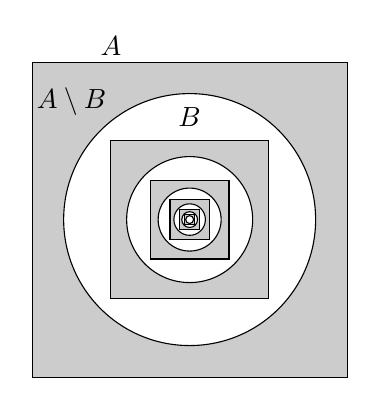
\begin{tikzpicture}
  \foreach \x in {1,0.5,0.25,0.25*0.5,0.25*0.25,0.25*0.25*0.5} {
    \path[draw,fill=black!20] (2*\x,2*\x)--(-2*\x,2*\x)--(-2*\x,-2*\x)--(2*\x,-2*\x)--cycle;
    \draw[fill=white] (0,0) circle (1.6*\x);
  };
  \node at (-1.0,2.2) {$A$};
  \node at (-1.5,1.5) {$A\setminus B$};
  \node at (0,1.3) {$B$};
  \node at (-0.75,0.75) {$$};
\end{tikzpicture}

  \caption{
  Nella dimostrazione del teorema di Cantor-Bernstein
  $A$ è rappresentato da un quadrato e $B$ da un cerchio contenuto
  in $A$. L'immagine di $A$ in $B$ è rappresentata da un quadrato contenuto
  in $B$ e così via. La parte ombreggiata è l'insieme $D$.
  }
  \label{fig:omotetia}
\end{figure}
%
\begin{proof}
Per prima cosa al posto dell'ipotesi $\# B \le \#A$ prendiamo
l'ipotesi apparentemente più forte $B\subset A$.
Vedremo alla fine che questa ipotesi non ci fa perdere di generalità.

Essendo per ipotesi $\#A \le \#B$ esiste $f\colon A \to B$ iniettiva.
Intuitivamente l'idea è quella di definire l'insieme
\[
 D = (A\setminus B)  \cup f(A\setminus B) \cup f^2(A\setminus B) \cup \dots
\]
e di definire la biezione $\phi \colon A \to B$ mandando ogni "buccia"
$f^n(A\setminus B)$ in $f^{n+1}(A\setminus B)$ e lasciando fisso
il resto di $B$.

Per farlo in maniera rigorosa
consideriamo allora la famiglia di insiemi $\F = \{X \subset A \colon X \supset A \setminus B, f(X) \subset X\}$ e definiamo $D = \bigcap \F$.
Osserviamo che $A \in \F$ quindi $\F\neq \emptyset$.

E' facile verificare che $f(D) \subset D$ infatti dato $x\in D$ per ogni $X\in \F$ deve essere $x\in X$ ma allora $f(x) \in X$ (per come è definito $\F$), dunque $f(x) \in D$. In modo analogo si dimostra che $D\supset A\setminus B$ e dunque concludiamo che $D\in \F$.

Verifichiamo ora che $f(D)=D\cap B$. Da un lato se $x\in D$ allora
$f(x) \in f(D)\subset D$ e $f(x)\subset f(A)\subset B$ da cui $f(x) \in D\cap B$.
Dall'altro lato se $y\in D \cap B$ e non fosse $y \in f(D)$
allora potremmo considerare l'insieme $X=D\setminus\{y\}$
e osservare che $X\in \F$.
Infatti in primo luogo $X \supset A \setminus B$ in quanto $D$ ha questa proprietà e $y \in B$.
Inoltre dato qualunque $x \in X$ visto che $X\subset D$ allora
$f(x) \in f(D)$ e, per ipotesi,
$y\not \in f(D)$ dunque $f(x)\neq y$ da cui $f(x) \in X$.
Dunque $X\in \F$ ma allora dovrebbe essere $D\subset X$ mentre
per costruzione abbiamo $y\in D$ ma non in $X$.

% Avendo visto che $f(D)=D\cap B$ possiamo facilmente
% osservare che $f(A\setminus D) \subset A \setminus D$.
% Infatti $f(A\setminus D)\subset f(A)=B$ e quindi
% $f(A\setminus D)\cap D \subset D \cap B = f(D)$
% ma essendo $f$ iniettiva si deve avere
% $f(A\setminus D) \cap f(D)=\emptyset$.

Possiamo allora definire $\phi \colon A \to B$
\[
\phi(x) =
\begin{cases}
   f(x) & \text{se $x\in D$}, \\
   x & \text{altrimenti.}
\end{cases}
\]
Chiaramente $\phi$ è iniettiva in quanto $f$ è iniettiva e manda $D$ in $D$
e l'identità è iniettiva e manda $A\setminus D$ in $A\setminus D$.

Per dimostrare che $\phi$ è suriettiva consideriamo qualunque $y \in B$.
Se $y\not \in D$ allora $\phi(y)=y$.
Se invece $y\in D$ essendo $y\in D\cap B = f(D)$ esisterà $x\in D$ tale
che $\phi(x) = f(x) = y$.

Abbiamo dimostrato il teorema nel caso $B\subset A$.
Nel caso generale sappiamo che esiste $f\colon A\to B$ iniettiva
ed esiste $g\colon B\to A$ iniettiva. Definiamo $\tilde B=g(B)$ e
definiamo $\tilde f\colon A\to \tilde B$ tramite $\tilde f(x) = g(f(x))$.
Chiaramente $\tilde B\subset A$ e $\tilde f$ è iniettiva.
Dunque ci siamo ricondotti alle ipotesi particolari e sappiamo che esiste
$\tilde \phi \colon A \to \tilde B$ biettiva. Ma allora possiamo definire
$\phi\colon A\to B$ come $\phi(x) = g^{-1}(\tilde \phi(x))$.
Essendo $\tilde \phi(A)=\tilde B$ ed essendo $g\colon B\to \tilde B$
invertibile, risulta che anche $\phi$ sia biettiva.
\end{proof}

% Il seguente teorema è vero se assumiamo l'assioma della scelta.
% \begin{theorem}
% Almeno una delle due relazioni è valida: $\#A \le \#B$ o $\#B \le \#A$.
% \end{theorem}

Il seguente teorema è rilevante in quanto ci dice che gli insiemi infiniti
non sono sempre tra loro equipotenti, ma ci sono infiniti più grandi e più piccoli.
Osserviamo inoltre che il paradosso di Russel
ricalca la dimostrazione di questo teorema.

\begin{theorem}[Cantor]
Per qualunque insieme $X$ si ha $\# X < \# \P(X)$.
\end{theorem}
%
\begin{proof}
Che sia $\#X\le \#\P(X)$ è facile, basta prendere la funzione
$f\colon X\to \P(X)$ definita da $f(x) = \{x\}$ e verificarne
l'iniettività.

Per mostrare che $\# X \neq \#P(X)$ consideriamo
$f\colon X \to \P(X)$ una qualunque funzione
e definiamo l'insieme
\[
   C = \{x \in X \colon x \not \in f(x) \}.
\]
Vogliamo ora mostrare che non esiste un $c\in X$ tale che $f(c) = C$.
Infatti se tale $c$ esistesse, si avrebbe che la proposizione
$c\in C$ risulterebbe equivalente a $c\not \in C$ il che è impossibile.
Dunque la funzione $f$ non può essere surgettiva e questo significa che
non è $\#X \le \#P(X)$.
\end{proof}

\begin{definition}
Dato $n\in \NN$ definiamo $I_n = \{k\in \NN\colon k < n\}$
(ad esempio $I_3=\{0,1,2\}$ è un insieme formato da $3$ elementi).
Se $A$ è un insieme diremo che $\# A= n$ se $\# A = \# I_n$.
Diremo in tal caso che $A$ ha $n$ elementi.
\end{definition}

Se vogliamo che la definizione precedente abbia senso,
dobbiamo assicurarci che $\# I_m = \# I_n$ se e solo se $m=n$.
Questo fatto apparentemente ovvio richiede una dimostrazione
un poco articolata. Cominciamo con il seguente.

\begin{lemma}\label{lemma:3834}
  Se $\# I_m \le \# I_n$ allora $m\le n$.
\end{lemma}
%
\begin{proof}
  Dimostreremo per induzione su $n$ la seguente proprietà:
  \[
    P(n)\colon \forall m\in \NN\colon \enclose{\#I_m\le \#I_n}\implies m\le n.
  \]

Verifichiamo se $P(0)$ è vera. Se $\#I_m\le \#I_0$ significa che esiste una
funzione iniettiva $f\colon I_m \to I_0 = \emptyset$. Ma non esistono funzioni
a valori nell'insieme vuoto, a meno che anche il dominio non sia vuoto. Dunque
$I_m=\emptyset$ e $m=0$ da cui segue ovviamente $m\le n$. Dunque $P(0)$ è vera.

Supponiamo per ipotesi induttiva che $P(n)$ sia vera e consideriamo $P(n+1)$.
Sia dunque $f\colon I_m \to I_{n+1}$ una funzione iniettiva.

Come primo passo vogliamo dimostrare che esiste una funzione iniettiva
$g\colon I_m \to I_{n+1}$ tale che $g(m-1)=n$.
Per fare ciò consideriamo due casi a seconda che $n\in f(I_m)$
oppure $n\not \in f(I_m)$.
Il secondo caso è più facile perché se $n\not \in f(I_m)$ basterà definire
\[
  g(k) =
  \begin{cases}
    f(k) & \text{se $k<m-1$}\\
    n & \text{se $k=m-1$}.
  \end{cases}
\]
La funzione $g$ così definita è certamente iniettiva in quanto $f$ lo è e il
valore $n$ non era già stato utilizzato da $f$.
Nel primo caso si avrà invece $f(j)=n$ per qualche $j<m$.
Se $j=m-1$ abbiamo finito perché $f(m-1)=n$ e basterà quindi scegliere $g=f$.
Se invece $j\neq m-1$ basterà scambiare i valori di $f$ nei punti $j$ e $m-1$:
\[
g(k) =
\begin{cases}
  f(k) & \text{se $k\neq j$ e $k\neq m-1$};\\
  f(m-1) & \text{se $k=j$};\\
  n & \text{se $k=m-1$}.
\end{cases}
\]
E' chiaro che $g$ rimane iniettiva se $f$ lo era.

Abbiamo quindi una funzione $g\colon I_m \to I_{n+1}$ iniettiva e tale
che $g(m-1)=n$. Significa che la restrizione $h = g_{|I_{m-1}}$ è una funzione
$h\colon I_{m-1}\to I_n$ in quanto il valore $n$ non viene mai assunto da $h$.
Ma allora ad $h$ si applica l'ipotesi induttiva e possiamo quindi affermare che
$m-1\le n$ da cui si ottiene immediatamente $m\le n+1$ come volevamo dimostrare.
\end{proof}

Dal lemma segue che se $\# I_m = \# I_n$ allora $m\le n$ e $n\le m$ e quindi $m=n$.
Viceversa è chiaro che se $m=n$ allora $\# I_n = \#I_m$ in quanto in tal caso
$I_m = I_n$.

\begin{exercise}\label{ex:9478}
Utilizzando il principio di induzione dimostrare che se $\# A = n$ allora:
\begin{enumerate}
    \item $\# \P(A) = 2^n$;
    \item $\# (A!) = \# \{f\colon A \to A\colon \text{$f$ biettiva}\} = n!$
      (le funzioni biettive di un insieme in sé si chiamano anche
      \emph{permutazioni});
    \item se $\# B = m$ allora $\# B^A = \#\{f\colon A \to B\} = m^n$.
\end{enumerate}
\end{exercise}

\begin{theorem}[unicità di $\NN$]
  Se $\NN$ e $\NN'$ sono due insiemi che soddisfano gli assiomi di Peano
  con $0\in \NN$, $0'\in \NN'$ e $\sigma\colon \NN \to \NN$ e
  $\sigma'\colon \NN' \to \NN'$ allora esiste una bigezione
  $\phi\colon \NN \to \NN'$
  tale che
  \[
    0'=\phi(0), \qquad \sigma'(\phi(n)) = \phi(\sigma(n)).
  \]
  Potremmo quindi dire che $\NN'$ è una copia \emph{isomorfa} di $\NN$.
  In particolare $\#\NN' = \# \NN$: gli insiemi che soddisfano gli
  assiomi di Peano hanno tutti la stessa cardinalità.
\end{theorem}
%
\begin{proof}
Possiamo definire $\phi\colon \NN \to \NN'$ per induzione:
\[
\begin{cases}
      \phi(0) = 0',\\
      \phi(\sigma(n)) = \sigma'(\phi(n))
\end{cases}
\]
e allo stesso modo possiamo definire $\psi\colon \NN'\to \NN$:
\[
\begin{cases}
      \psi(0') = 0,\\
      \phi(\sigma'(n)) = \sigma(\psi(n)).
\end{cases}
\]
A questo punto è facile verificare per induzione che $\psi(\phi(n)) = n$ per
ogni $n\in \NN$. Invertendo i ruoli di $\phi$ e $\psi$ si dimostra allo stesso
modo che $\phi(\psi(n))=n$ per ogni $n\in \NN'$.
Significa che $\psi$ è l'inversa di $\phi$
e che quindi $\phi$ è bigettiva.
\end{proof}

\section{Insiemi finiti/infiniti}

L'insieme dei numeri naturali è, per certi versi, paradossale, come si può
capire dalla seguente storiella.

\begin{exercise}[Hotel Hilbert]\index{Hotel Hilbert}
  Nell'hotel Hilbert, come in tutti gli hotel, ogni stanza ha associato univocamente
  un numero naturale: il numero della stanza.
  Però a differenza degli altri hotel nell'hotel Hilbert c'è una stanza per
  ogni numero naturale, quindi le stanze e i numeri naturali sono in corrispondenza
  biunivoca (diremo quindi che ci sono \emph{infinite} stanze).

  Un bel giorno arriva un cliente all'hotel e chiede all'addetto
  alla \emph{reception} di avere una stanza. Purtroppo l'hotel è pieno e
  quindi l'addetto informa il cliente che non è possibile avere una stanza.
  Il cliente insiste e fa chiamare il direttore che risolve la questione in
  maniera assolutamente brillante.
  Il direttore chiede gentilmente ad ogni ospite dell'hotel di spostarsi dalla sua
  stanza a quella seguente. Cioè: l'ospite nella stanza $n$ si deve spostare nella
  stanza $n+1$. In tal modo si libera la stanza numero $0$ che quindi può essere
  utilizzata dal nuovo arrivato.

  Il giorno seguente arriva all'albergo una corriera che porta infinite persone,
  una per ogni numero naturale, come per l'albergo. Ma l'albergo è già pieno.
  Come farà il direttore a fare spazio per tutte queste persone?
\end{exercise}

In realtà non c'è niente di paradossale nella storiella precedente, se non il
fatto che vogliamo ragionare con insiemi infiniti.
L'esistenza della funzione $\sigma$ può anzi essere presa come definizione
di insieme infinito.

\begin{definition}
  Diremo che un insieme $A$ è \myemph{finito}
  se esiste $n\in \NN$ tale che $\#A = n$.
  Diremo che un insieme $A$ è \myemph{infinito} (più precisamente si direbbe
  \emph{Dedekind infinito})
  se esiste una funzione $\sigma\colon A \to A$
  iniettiva ma non suriettiva.
\end{definition}

Chiaramente $\NN$ (se esiste) è un esempio di insieme infinito in quanto
la funzione successore $\sigma(n) = n+1$ è iniettiva ma non suriettiva
su $\NN$. E' anche facile verificare che se $\#A \ge \#\NN$ allora $A$
è infinito (lo si provi per esercizio).

Viceversa si ha il seguente teorema che afferma, sostanzialmente,
che ogni insieme infinito contiene una copia di $\NN$ e dunque $\NN$ è,
in un certo senso, il più piccolo insieme infinito.

\begin{theorem}\label{th:4994}
  Se $A$ è un insieme infinito allora esiste un insieme $N\subset A$
  che soddisfa
  gli assiomi di Peano e quindi $\#A \ge \#\NN$.
\end{theorem}
%
\begin{proof}
  Sia $\sigma\colon A \to A$ una funzione iniettiva ma non suriettiva.
  Scegliamo un punto $0\in A \setminus \sigma(A)$ e definiamo
  \[
    \mathcal F = \{ X\subset A\colon 0\in X, x\in X \implies \sigma(x)\in X\}.
  \]
  Sostanzialmente $\mathcal F$ è l'insieme dei sottoinsiemi di $A$ che soddisfano
  l'assioma di induzione di Peano.
  Definiamo quindi
  \[
    N = \bigcap \mathcal F.
  \]
  Chiaramente $N\in \mathcal F$ (verificare!) e quindi $N$ soddisfa tutti
  gli assiomi
  di Peano scelto $0\in N$  come zero e
  $\sigma_{|N}\colon N \to N$ come funzione successore.
\end{proof}

Per quanto riguarda gli insiemi finiti abbiamo il seguente risultato che ci
assicura, in particolare, che gli insiemi finiti non sono infiniti.

\begin{theorem}
Se $A$ è finito e $f\colon A \to A$ è una funzione allora
risultano equivalenti
\begin{enumerate}
  \item $f$ è iniettiva;
  \item $f$ è surgettiva;
  \item $f$ è bigettiva.
\end{enumerate}
\end{theorem}
%
\begin{proof}
  Se $A$ è finito significa che esiste $n\in \NN$ tale che $A$ è in
  corrispondenza biunivoca con $I_n$. Potremo quindi supporre, senza
  perdere di generalità, che sia $A=I_n$.

  Supponiamo per assurdo che esista una funzione iniettiva ma non suriettiva
  $f\colon I_n \to I_n$.
  Se fosse $n\not \in f(I_n)$ si avrebbe $f\colon I_n \to I_{n-1}$ iniettiva,
  da cui, per il Lemma~\ref{lemma:3834} avremmo $n\le n-1$ assurdo.
  Ma se anche fosse $n=f(k)$ per qualche $k\in I_n$
  dovrebbe allora esistere $x\in I_n\setminus f(I_n)$
  e sarebbe $x\neq n$.
  Allora
  potrei definire $g\colon I_n\to I_{n-1}$ che redireziona in $x$ il punto
  che prima andava in $n$:
  \[
    g(j) =
    \begin{cases}
      f(j) & \text{se $j\neq k$},\\
      x & \text{se $j=k$.}
    \end{cases}
  \]
  Chiaramente $g\colon I_n\to I_{n-1}$ sarebbe iniettiva
  e di nuovo otterremmo un assurdo.

  Abbiamo mostrato che se $f$ è iniettiva allora $f$ è anche suriettiva e dunque
  anche bigettiva.

  Viceversa consideriamo una funzione surgettiva $f\colon I_n \to I_n$.
  Possiamo allora definire $g\colon I_n\to I_n$
  \[
    g(n) = \min f^{-1}({n}).
  \]
  Visto che $f$ è surgettiva, $f^{-1}(\{n\})$ non è mai vuoto e quindi
  $g$ è ben definita su tutto $I_n$. Risulta inoltre che $g$ è iniettiva
  in quanto $f^{-1}(\{n\}) \cap f^{-1}(\{m\}) = \emptyset$ se $m\neq n$.
  Per quanto visto prima $g$ deve però essere anche surgettiva e questo
  significa che $f^{-1}(\{n\})$ contiene un unico elemento.
  Ma allora $f$ era anche iniettiva. Abbiamo quindi mostrato che se
  $f$ è surgettiva allora è anche iniettiva e quindi anche bigettiva.
\end{proof}

\begin{theorem}
  Se $A$ è finito e $B\subset A$ allora anche $B$ è finito.
\end{theorem}
%
\begin{theorem}
  Dimostriamo per induzione su $n$ che se $\#A = n$ allora ogni $B\subset A$
  è finito.
  Per $n=0$ si nota che $\#A = 0$ implica $A=\emptyset$ e quindi $B=\emptyset$
  è certamente finito.
  Supponiamo ora che sia $\#A = n+1$ e consideriamo $B\subset A$.
  Se $B=A$ allora ovviamente $\#B=\#A=n+1$ e quindi $B$ è finito.
  Altrimenti esiste $x\in A\setminus B$. E' facile verificare che
  $\#(A\setminus\{x\}) = n$ ed essendo $B\subset A\setminus\{x\}$
  applicando l'ipotesi induttiva si ottiene che $B$ è finito.
\end{theorem}

Viceversa si può dimostrare il seguente risultato.
\begin{theorem}
  Un insieme è finito oppure infinito.
\end{theorem}
%
\begin{proof}
Se $\# A \ge \#\NN$ allora esiste una funzione iniettiva $f\colon \NN \to A$
e sappiamo esistere una funzione iniettiva ma non surittiva $\sigma\colon \NN \to \NN$.
Posto $B=f(\NN)$ si ha dunque che $f\colon \NN\to B \subset A$ è bigettiva.
Dunque possiamo definire $g \colon A \to A$ come
\[
g(a) =
\begin{cases}
    a & \text{se $a\not \in B$}\\
    f(\sigma(f^{-1}(a))) & \text{se $a \in B$}.
\end{cases}
\]
Non è difficile verificare che $g$ è iniettiva ma non suriettiva in quanto
l'elemento $f(0)$
non viene mai raggiunto da $g$. Dunque se $\# A \ge \#\NN$ certamente $A$
è infinito.

Ora mediante l'assioma della scelta si potrebbe dimostrare che se non è
$\#A \ge \#\NN$ allora necessariamente si ha $\#A < \#\NN$
(non lo dimostriamo perché richiederebbe diverse nuovi nozioni).
Ma se $\#A < \#\NN$ allora esiste una funzione iniettiva $f\colon A \to \NN$.
Poniamo $B=f(A)$ cosicché $f\colon A \to B$ è bigettiva. Per dimostrare
che $A$ è finito basterà allora dimostrare che $B\subset \NN$ è finito.

Se esiste $n\in \NN$ tale che $B\subset I_n$ allora si avrebbe $\#A\le \#I_n$
e dunque $A$ sarebbe finito perché in corrispondenza biunivoca con un sottoinsieme
di un insieme finito. Supponiamo allora che per ogni $n\in \NN$ si abbia
$B\setminus I_n\neq \emptyset$. Costruiamo allora una funzione
$f\colon \NN \to B$ tramite la seguente definizione ricorsiva:
\[
 \begin{cases}
    f(0) = \min B \\
    f(n+1) = \min (B\setminus I_{f(n)+1}).
 \end{cases}
\]
La funzione è ben definita perché $B$ e $B\setminus I_m$ non sono mai vuoti
e il buon ordinamento di $\NN$ garantisce l'esistenza del minimo.
E' chiaro che $f(n+1) > f(n)$ e dunque (lo si potrebbe dimostrare per induzione)
la funzione $f$ è iniettiva. Significa dunque che $\NN\le A$ contro l'ipotesi
$\#A < \#\NN$.

\end{proof}

\section{Ennuple e successioni}

Abbiamo denotato con $B^A$ l'insieme delle funzioni $f\colon A \to B$ e
abbiamo denotato con $I_n = \{1, 2, \dots, n-1\} = \{k\in \NN \colon k<n\}$.
Se $A$ è un insieme qualunque e $n\in\NN$ definiamo allora:
\[
   A^n = A^{I_n} = \{\vec a\colon \{1, 2, \dots, n-1\}\to A\}.
\]
Gli elementi $\vec a \in A^n$ vengono chiamate $n$-uple (ennuple) perché
sono identificate dagli $n$ valori che assumono sugli $n$ numeri $0,1,\dots,n-1$.
Normalmente si utilizza la notazione $a_k = \vec a(k)$ per denotare
il $k$-esimo valore assunto dalla funzione $\vec a$ e si scriverà:
\[
  \vec a = (a_0, a_1, \dots, a_{n-1}).
\]
Gli elementi (di solito saranno numeri) $a_0$, $a_1$, \dots, $a_{n-1}$ vengono
chiamati componenti della ennupla $\vec a$. I pedici $0,1, \dots, n-1$ vengono
chiamati \emph{indici}.

Noi utilizzeremo la convenzione di usare simboli in \emph{grassetto} per denotare
le ennuple. Nella scrittura a mano (dove il grassetto è impraticabile)
si scriverà $\underline{a}$ al posto di $\vec a$. Un'altra alternativa (meno comoda)
è $\stackrel{\to}{a}$.
La notazione è quella utilizzata in fisica per denotare i \emph{vettori} perché,
in effetti, se mettiamo una base in uno spazio vettoriale di dimensione finita
ogni vettore può essere identificato dalla ennupla delle sue componenti rispetto
alla base.

Ad esempio l'ennupla $\vec a = (3,5,3)$ è elemento di $\NN^3$.
Sarà $\vec a = (a_0, a_1, a_2)$ con $a_0=3$, $a_1=5$, $a_2=3$.
Formalmente $\vec a$ è definita come una funzione:
$\vec a = \{0\mapsto 3, 1\mapsto 5, 2 \mapsto 3\}$ ma in pratica non è importante
quale sia la definizione (altri testi potrebbero dare definizioni diverse ma equivalenti)
ma solo quali siano le sue proprietà.
E' anche consuetudine utilizzare gli indici a partire da $1$ invece che da $0$
e quindi spesso si troverà scritto $\vec a = (a_1, a_2, a_3)$.

Osserviamo che se $n=2$ la notazione utilizzata per le ennuple $A^2$ è la stessa
notazione utilizzata per le coppie $A\times A$.
L'ambiguità è giustificata dal fatto che si potrebbe in effetti identificare
$A^2$ con $A\times A$ in quanto gli elementi di $A^2$ soddisfano la proprietà
caratterizzante le coppie:
\[
  (x,y) = (x',y') \iff (x=x') \land (y=y').
\]
Osserviamo che formalmente $(A\times A)\times A \neq A^3$ in quanto gli elementi
del primo insieme sono coppie del tipo $((x,y),z)$ mentre gli elementi
del secondo insieme sono $3$-uple (triple) della forma $(x,y,z)$.
E' chiaro quindi che pur essendo oggetti diversi possono essere messi
in corrispondenza tra loro.

In maniera analoga chiameremo \emph{successioni} a valori in $A$ gli
elementi dell'insieme
\[
  A^\NN = \{\vec a\colon \NN \to A\}.
\]
Di nuovo useremo la notazione $a_k = \vec a(k)$ per denotare i valori
della successione $\vec a$ e scriveremo, in maniera espressiva:
\[
  \vec a = (a_0, a_1, a_2, \dots, a_n, \dots).
\]
Gli elementi $a_0, a_1, \dots$ vengono chiamati \emph{termini} o \emph{valori}
della successione. I pedici $0,1,\dots$ vengono chiamati \emph{indici} come per
le ennuple.

Per scrivere una successione a partire dai suoi termini
si può usare la notazione $\vec a = (a_n)_{n\in \NN}$ o
$\vec a = (a_n \colon n \in \NN)$
o anche
$\vec a = (a_n)_{n=0}^{+\infty}$. In queste notazioni la variabile $n$ è muta.
Spesso tali notazioni si abbreviano in una
notazione (formalmente impropria) $\vec a = (a_n)$ o anche $\vec a = a_n$.

Per esempio la funzione $\vec a (n) = n^2$ definisce la successione dei quadrati:
\[
 \vec a = (0,\ 1,\ 4,\ 9,\ 16,\ \dots, n^2,\ \dots).
\]
Ma più spesso si dirà: consideriamo la successione $a_n = n^2$ indicando il
termine generico invece dell'intera successione.

Deve essere chiaro che la successione $(a_n)_{n\in \NN}$ è cosa diversa
dall'insieme dei suoi valori $\{a_n\colon n\in \NN\}$.
Ad esempio
le successioni con termini
\[
a_k = \begin{cases}
      1 & \text{se $k=0$}\\
      0 & \text{se $k>0$}
      \end{cases},
       \qquad
b_k = \begin{cases}
     0 & \text{se $k=0$}\\
     1 & \text{se $k>0$}
     \end{cases},
\]
sono successioni diverse ma hanno lo stesso insieme di valori
\[
\{a_k\colon k\in \NN\} = \{b_k \colon k\in \NN \} = \{ 0, 1\}.
\]
La differenza sta nel fatto che in un insieme gli elementi non sono ordinati
e non contano le ripetizioni,
nelle succesioni invece (come nelle coppie e nelle ennuple) conta l'ordine e
contano eventuali ripetizioni.

Ennuple e successioni potrebbero essere entrambe racchiuse dal termine
\emph{sequenze}.
Una ennupla sarebbe una sequenza finita, una successione una sequenza infinita.

\section{I numeri interi}

Dati due numeri naturali $n,m\in \NN$ vogliamo definire
il \emph{percorso} (o traslazione) $m\mapsto n$ necessario per
andare da $m$ a $n$. Se $n\ge m$ significa che $n$ si può ottenere da $m$ sommando
un certo numero naturale $k$: $n=m+k$. Il numero $k$ viene chiamato
\myemph{differenza} tra $n$ ed $m$. Se invece $n<m$ il percorso $m\mapsto n$
è il percorso \emph{opposto} di $n\mapsto m$ e la differenza è, in un senso
da precisare, l'opposto del numero $k$ tale che $m=n+k$.
A posteriori vedremo che il percorso $m\mapsto n$ rappresenta il numero intero
$n-m$.

Diremo che due percorsi $m\mapsto n$ e $m'\mapsto n'$
sono \emph{equivalenti} se la differenza è la stessa, ovvero se:
\[
  m + n' = m' + n.
\]
Se, ad esempio, $m'=m+k$ e $n'=n+k$ è chiaro che $m'\mapsto n'$ risulta
equivalente a $m\mapsto n$.
Ricordando che $m\mapsto n$ può essere rappresentato come una coppia
$(m,n)\in \NN\times \NN$ definiamo quindi la seguente relazione
$\sim$ su $\NN \times \NN$:
\[
  (m,n) \sim (m',n') \iff m + n' = m' + n.
\]

E' facile verificare che la relazione $\sim$ appena introdotta
è una relazione di equivalenza in base alla seguente definizione.

\begin{definition}[relazione di equivalenza]
  Una relazione $\sim$ su un insieme $A$ si dice essere una
  \myemph{relazione di equivalenza} se è una relazione
  riflessiva (cioé $x\sim x$),
  simmetrica (cioé $x\sim y \iff y\sim x$) e
  transitiva
  (cioé $(x \sim y) \land (y\sim z) \implies x \sim z$).
\end{definition}

Le relazioni di equivalenza permettono di definire un insieme
chiamato \emph{quoziente}.

\begin{definition}[insieme quoziente]
  Sia $\sim$ una relazione di equivalenza su un insieme $A$.
  Dato $a \in A$ definiamo la \myemph{classe di equivalenza di $a$}
  come l'insieme di tutti gli elementi di $A$ che sono in relazione
  con $a$:
  \[
   [a] = \{x \in A \colon x \sim a\}.
  \]
  L'insieme di tutte le classi di equivalenza viene chiamato
  \myemph{insieme quoziente}:
  \[
  A/{\sim} = \{[x] \colon x \in A\}.
  \]
  Dunque se $\alpha \in A/{\sim}$ deve esistere $a\in A$ tale che
  $\alpha = [a]$. In tal caso si dirà che $a$ è un
  \myemph{rappresentante}
  di $\alpha$.
\end{definition}

L'insieme quoziente serve a identificare come uguali
tutti gli elementi che sono tra loro equivalenti:
se $\sim$ è una relazione di
equivalenza allora si ha
\[
  x\sim y \iff [x]=[y].
\]

Infatti se $x \sim y$ e se $z\in [x]$ si ha $z\sim x \sim y$ e quindi $z\in
[y]$.
Dunque se $x\sim y$ si ha $[x]\subset [y]$ ma, scambiando i ruoli di $x$ e $y$
si avrà anche $[y]\subset [x]$ e quindi $[x]=[y]$. D'altra parte se $[x]=[y]$
essendo $x\sim x$ si ha $x\in [x] = [y]$ e quindi $x\sim y$.

Tornando alla relazione di equivalenza $\sim$ definita su $\NN\times \NN$
andremo quindi a definire:
\[
  \ZZ = (\NN \times \NN)/\sim.
\]

Ogni elemento di $\ZZ$ è dunque una classe di equivalenza di percorsi
$m\mapsto n$ tutti con la stessa direzione e lunghezza.

I percorsi possono essere sommati per \emph{concatenazione}. Se concateniamo
il percorso $m\mapsto n$ con $n\mapsto h$ otteniamo il percorso $m\mapsto h$.
In generale se vogliamo sommare $m\mapsto n$ con $m'\mapsto n'$
dobbiamo spostare uno dei due percorsi in modo che il suo punto di partenza coincida
con il punto di arrivo dell'altro. Se, ad esempio, si ha $m'\ge n$ troveremo $k\in \NN$
tale che $m'=n+k$ e dunque $(m,n)\sim(m+k,n+k)=(m+k,m')$ da cui
\[
  (m+k,m') + (m',n') = (m+k,n')
\]
e sommando $n$ alle due componenti del risultato si ottiene
$(m+k+n,n'+n) = (m+m,n+n')$.
In generale si può quindi verificare che la somma di due classi di equivalenza
di percorsi è sempre ben definita nel modo seguente:
\[
  [(m,n)] + [(m',n')] = [(m+m',n+n')].
\]
Si osserva che se al posto di $(m,n)$ mettiamo $(m+k,n+k)$ si ottiene
\[
  [(m+k,n+k)] + [(m',n')] = [(m+m'+k,n+n'+k)] = [(m+m',n+n')]
\]
cioè il risultato non cambia (se così non fosse la definizione non sarebbe
ben posta perché dipenderebbe dal rappresentante scelto).

E' facile verificare che l'addizione così definita gode delle proprietà:
associativa e commutativa.

Similmente vorremmo dire che il percorso $m\mapsto n$ è maggiore-o-uguale
del percorso $m\mapsto n'$ quando $n\ge n'$. Se due percorsi non partono
dallo stesso punto posso sempre spostarne uno dei due mantenendo l'equivalenza e
riconducendosi al caso in cui entrambi partono dallo stesso punto.
Procedendo in maniera analoga a quello che abbiamo fatto per la somma
si ottiene la segunte definizione per la relazione d'ordine $\le$:
\[
  [(m,n)] \le [(m',n')] \iff n+m' \ge n' + m.
\]

E' facile verificare che la relazione d'ordine così definita
gode della proprietà invariantiva:
\[
  i \ge j \iff i+k \ge j+k, \qquad \forall i,j,k\in \ZZ
\]
e più in generale è compatibile con la somma:
\[
 (i\ge j) \land (i'\ge j') \implies i+i' \ge j+j'.
\]

Se due percorsi sono equivalenti anche i percorsi opposti lo sono. Questo ci permette
di definire anche l'operazione di opposto (denotato con l'operatore unario $-$)
sulle classi di equivalenza:
\[
  -[(m,n)] = [(n,m)].
\]
Si osservi che sommando un percorso con l'opposto si ottiene la classe
di equivalenza del percorso nullo:
\[
  [(m,n)] + [(n, m)] = [(m+n,n+m)] = [(0,0)]
\]
e l'opposto dell'opposto è il percorso originario:
\[
  -(-[(m,n)]) = -[(n,m)] = [(m,n)].
\]

Un percorso $m\mapsto n$ può essere di tre tipi: \emph{positivo}
se $n>m$, \emph{negativo} se $n<m$ e \emph{nullo} se $m=n$.
Ogni percorso
positivo $m\mapsto n$ è equivalente ad un percorso del tipo $0\mapsto k$ dove
$k$ è la differenza tra $n$ ed $m$ ovvero $n=m+k$.
I percorsi \emph{positivi} sono quindi rappresentati dalla coppia $(0,k)$ con $k\in \NN$,
$k\neq 0$. Il percorso nullo è equivalente al percorso $0\mapsto 0$ e può quindi essere
rappresentato, come i percorsi positivi ponendo $k=0$, dalla coppia $(0,0)$.
I percorsi \emph{negativi} sono della forma $m\mapsto n$ con $n<m$. In tal caso esiste $k\in \NN$
tale che $m=n+k$ e il percorso può essere rappresentato dal suo equivalente $k \mapsto 0$ ovvero
dalla coppia $(k,0)$ con $k\in \NN$, $k\neq 0$.

Se chiamiamo $\NN'\subset \ZZ$ l'insieme delle classi di equivalenza
dei percorsi positivi o nulli potremo scrivere:
\[
  \NN' = \{[(0,k)]\colon k\in \NN\}.
\]
Si osserva allora che l'addizione ristretta a $\NN'$ si esegue
banalmente sommando la seconda componente su $\NN$:
\[
  [(0,k)] + [(0,j)] = [(0,k+j)]
\]
e l'ordinamento su $\NN'$ corrisponde all'ordinamento su $\NN$:
\[
  [(0,k)] \ge [(0,j)] \iff k \ge j.
\]
Significa che $\NN'$ è \emph{isomorfo} ad $\NN$ tramite la bigezione
$\NN\mapsto \NN'$ dato da $k\mapsto [(0,k)]$. Tale bigezione
preserva l'addizione e l'ordinamento e in questo senso diciamo che è un
isomorfismo. Il numero naturale $0\in \NN$ corrisponde in tale isomorfismo
al percorso nullo $[(0,0)]\in \NN'$.

In questo senso possiamo pensare che $\ZZ$ sia una estensione di $\NN$.
D'ora in poi chiameremo \emph{numeri interi} gli elementi di $\ZZ$
e penseremo ai numeri naturali come al sottoinsieme $\NN'$ dei numeri
interi.
Si ha infatti:
\[
  \ZZ = \NN' \cup (-(\NN'\setminus\{0\}))
\]
dove $\NN'$ sono dunque i numeri interi positivi o nulli, $\NN'\setminus\{0\}$
sono i numeri interi positivi $-(\NN'\setminus\{0\})$ sono i numeri interi
negativi.

Visto che $\NN$ era un qualunque insieme soddisfacente gli assiomi di Peano
e visto che anche $\NN'$ come $\NN$ soddisfa gli assiomi di Peano,
potremo d'ora in poi dimenticare il vecchio $\NN$ e utilizzare $\NN'$ al suo
posto chiamandolo, d'ora in poi $\NN$. Supporremo dunque che sia
$\NN \subset \ZZ$.

Dunque abbiamo $0,1,2,\dots \in \ZZ$ ma anche $-1,-2,-3, \dots \in \ZZ$.
Dalle definizioni precedenti è facile osservare che $-0=0$.

Oltre all'addizione e all'ordinamento che abbiamo estesi da $\NN$ a $\ZZ$,
su $\ZZ$ possiamo definire l'operazione di \emph{sottrazione} (denotata con
l'operatore binario $-$) come segue:
\[
  a-b = a + (-b).
\]
Osserviamo inoltre che l'opposto $-a$ di un intero $a\in \ZZ$ è l'unico
intero tale che
\[
  a + (-a) = 0
\]
e dunque in generale $a-a=0$.

Su $\NN$ avevamo definito anche l'operazione di moltiplicazione e vogliamo
estendere anch'essa a tutto $\ZZ$.
Avendo identificato $\NN$ con $\NN'$ ora scriveremo $n-m$ al posto di $[(m,n)]$.
Se vogliamo mantenere la proprietà distributiva del prodotto rispetto alla somma
dovrà essere, per ogni $n\in \NN$:
\[
  0 = 0\cdot n = (1+(-1))\cdot n = 1\cdot n + (-1)\cdot n
   = n + (-1)\cdot n
\]
da cui si ottiene che $(-1)\cdot n$ è l'opposto di $n$, ovvero:
\[
  -n = (-1)\cdot n.
\]
Analogamente dovrà essere $n\cdot (-1) = -n$.

Allora se $n,m\in \NN$ e se vogliamo mantenere la proprietà associativa
della moltiplicazione dovremo avere:
\[
  n \cdot (-m) = n \cdot (-1) \cdot m = (-n)\cdot m = (-1)\cdot (n\cdot m)
   = -(n\cdot m)
\]
(più per meno: meno)
e
\[
(-n)\cdot(-m) = (-1) \cdot n \cdot (-1) \cdot m = (-1)(-n)\cdot m
 = (-(-n))\cdot m = n\cdot m
\]
(meno per meno: più).
Sulle classi di equivalenza potremo quindi definire
la moltiplicazione come segue:
\[
[(m,n)]\cdot [(m',n')] = [(n\cdot n' + m\cdot m',n\cdot m' + n'\cdot m)].
\]
Si potrà quindi verificare che cambiando i rappresentanti scelti per le
classi (ad esempio sostituendo $(m,n)$ con $(m+k,n+k)$) il risultato non
cambia (si utilizzerà la proprietà distributiva su $\NN$).
Si potrà quindi verificare che la moltiplicazione così definita su $\ZZ$
estende la moltiplicazione di $\NN$ e continua a mantenere le proprietà associativa,
commutativa e distributiva.

Chiaramente su $\ZZ$ come avevamo fatto su $\NN$ oltre alla relazione d'ordine
$\ge$ si definiscono conseguentemente le relazioni d'ordine stretto $>$ e
le relazioni inverse $\le$ e $<$.
Risulta che gli interi positivi sono gli $n\in \ZZ$ tali che $n>0$ e gli
interi negativi sono gli $n\in \ZZ$ tali che $n<0$.

Su $\ZZ$ definiamo anche la funzione \emph{valore assoluto}
\[
  \abs{n} =
  \begin{cases}
      n & \text{se $n\ge 0$}\\
      -n & \text{se $n<0$}
  \end{cases}.
\]
L'immagine di tale funzione definita su $\ZZ$ è $\NN$.

\section{Divisibilità e numeri primi}

Se $n,m\in \ZZ$ e se esiste $k\in \ZZ$ tale che $m=k\cdot m$
diremo che $n$ \myemph{divide} $m$,
che $m$ è un \myemph{divisore} di $n$
e scriveremo $n\mid m$.
Ad esempio se $2\mid n$ diremo che $n$ è \myemph{pari}, altrimenti diremo che $n$
è \myemph{dispari}.
Visto che $n = 1\cdot n$ è chiaro che $1$ e $n$ sono sempre divisori di $n$
(e anche $-1$ e $-n$ lo sono).

Definiamo il \emph{massimo comun divisore} di due numeri $n,m$ come
\[
  MCD(n,m) = \max \{k\in \NN\colon (k\mid n) \land (k \mid m)\}.
\]
Tale massimo esiste perché l'insieme preso in considerazione
è non vuoto (contiene sempre il numero $1$) ed è finito perchè


Se $n=k\cdot m$ con $k\neq \pm 1$ (cioè $k\neq 1$ e $k\neq -1$)
diremo che $n$ è \emph{riducibile}.
In caso contrario diremo
che $n$ è \emph{irriducibile}.

\begin{theorem}[teorema fondamentale dell'aritmetica]
  Ogni $n\in \NN$, $n\ge 2$, può essere scritto nella forma:
  \begin{equation}\label{eq:48273}
    n = p_1 \cdot p_2 \cdot \ldots \cdot p_N
  \end{equation}
  dove tutti i $p_k$ sono irriducibili e
  $2 \le p_1 \le p_2 \le \dots \le p_N$.
  Inoltre i $p_k$ sono univocamente determinati (la
  decomposizione~\eqref{eq:48273} è unica).

  L'espressione \eqref{eq:48273} viene chiamata \myemph{fattorizzazione}
  di $n$ (in quanto gli operandi della moltiplicazione
  si chiamano \emph{fattori}).
\end{theorem}
%
\begin{proof}
  Dimostriamo per induzione su $m$ il seguente
  $P(m)$: ``ogni naturale $n<m$, $n\ge 2$
    ammette una unica decomposizione
    nella forma \eqref{eq:48273}''.

  L'enunciato è banalmente vero per $m=3$ in quanto l'unico $n$ in questione
  è $n=2$ e se $k,j\ge 2$ allora
  $k\cdot j\ge 4$ e quindi $n=2$ non può essere scritto come prodotto di due
  naturali non inferiori a $2$.
  Significa che $2$ è irriducibile e può essere scritto in modo unico come $2=2$
  (prodotto di un unico irriducibile).

  Supponiamo ora di sapere che vale $P(m)$ e dimostriamo $P(m+1)$.
  E' sufficiente dimostrare che $n=m$ può essere scritto in modo unico
  nella forma~\eqref{eq:48273} (in quanto se $n<m$ il risultato è garantito
  dall'ipotesi induttiva $P(m)$).
  Sia $p_1 = \min\{p\ge 2\colon p|n\}$.
  Tale minimo esiste certamente perché l'insieme non è vuoto visto che contiene
  quantomeno il numero $n$. Inoltre $p_1$ è certamente irriducibile perché se
  $p_1$ avesse a sua volta un divisore $p$ allora anche $p$ sarebbe un divisore
  di $n$ e sarebbe $p<p_1$ contro l'ipotesi che $p_1$ fosse il minimo.
  Visto che $p_1\mid n$ esiste $n'$ tale che $n=p_1\cdot n'$.
  Visto che $p_1>1$ certamente è $n'<n=m$ e dunque applicando $P(m)$ sappiamo
  che $n'$ ammette una unica decomposizione che possiamo scrivere nella forma:
  \[
    n' = p_2 \cdot p_3 \dots p_N
  \]
  (abbiamo utilizzato gli indici a partire da $2$ invece che da $1$ perché $p_1$
  è già stato utilizzato). Dunque avremo che
  \[
    n = p_1 \cdot n' = p_1 \cdot p_2 \dots p_N
  \]
  come volevamo dimostrare. L'unica cosa che rimane da verificare è che
  sia $p_1\le p_2$. Ma visto che $p_2 \mid n'$ e $n'\mid n$ scopriamo che
  $p_2\mid n$ e quindi essendo $p_1$ il minimo divisore di $n$ deve essere
  $p_1\le p_2$.
\end{proof}

Un numero $p$ si dice essere \myemph{primo}
se ogni volta che $p$ divide un prodotto esso divide almeno uno dei due fattori
cioè se per ogni $n,m\in \ZZ$ si ha:
\[
  p \mid m\cdot n \implies (p\mid m)\lor(p\mid n).
\]

Il prossimo teorema ci dice che sui numeri interi \emph{primo} e \emph{irriducibile} sono sinonimi (e spesso la definizione di numero primo viene espressa mediante irriducibilità) ma in contesti più generali si possono distinguere i due concetti.

\begin{theorem}
Un numero  $p\in \ZZ$ è primo se e solo se è irriducibile.
\end{theorem}
%
\begin{proof}
Supponiamo che $p$ sia primo e che si possa scrivere $p=n\cdot m$ con $n,m\in\ZZ$.
Allora chiaramente $p\mid n\cdot m$ e quindi $p$ divide almeno uno tra $n$ e $m$.
Senza perdita di generalità possiamo supporre $p\mid n$ da cui $p=p\cdot m$.
Significa quindi che $m=1$ e quindi $p$ non è riducibile.

Viceversa supponiamo che $p$ sia irriducibile e supponiamo che $p\mid n\cdot m$.
Per il teorema fondamentale dell'aritmetica $n$ e $m$ hanno una unica
fattorizzazione e il prodotto delle fattorizzazioni mi dà una fattorizzazione
di $n\cdot m$. D'altra parte la fattorizzazione di $p$ è $p$ stesso in quanto
$p$ è irriducibile. Dunque se $p\mid n\cdot m$ necessariamente $p$ è uno dei
termini della fattorizzazione di $n\cdot m$ ma visto che tale fattorizzazione
si ottiene moltiplicando tra loro le fattorizzazioni di $n$ e di $m$,
si deduce che $p$ è in una delle due fattorizzazioni e quindi divide
uno tra $n$ e $m$.
\end{proof}

\section{I numeri razionali}

In maniera simile a come abbiamo ottenuto gli interi estendendo i naturali in
modo da poter invertire l'operazione di addizione, vogliamo estendere gli
inter in modo da poter invertire l'operazione di moltiplicazione.
Dati due interi $p,q$ con $q\neq 0$,
consideriamo la \emph{dilatazione} $q\mapsto p$ che
lascia fisso lo $0$, manda $q$ in $p$ e manda ogni multiplo di $q$ ovvero
ogni intero $n$ della forma $n=kq$ in $kp$.
Chiamiamo \myemph{frazione} la coppia $q\mapsto p$ che denoteremo più espressivamente
nella forma $\frac{p}{q}$.
Nella frazione $\frac{p}{q}$ il numero $p$ viene chiamato \myemph{numeratore}
e il numero $q$ \myemph{denominatore}.
Sulle frazioni possiamo mettere una relazione di equivalenza.
In effetti se $p'=kp$ e $q'=kq$ con $k\in \ZZ$, $k\neq 0$,
le dilatazioni $q\mapsto p$ e $q'\mapsto p'$
agiscono nello stesso modo sui multipli di $q'$.
Infatti se $n=jq'=kjq$ la dilatazione $q\mapsto p$ lo manda in $kjp$ e
la dilatazione $q'\mapsto p'$ lo manda in $jp'=kjp$.
Se $q'=kq$ e $p'=kp$ allora equivalentemente si ha $pq'=p'q$.
Definiamo quindi la relazione di equivalenza tra frazioni:
\[
  \frac{p}{q} \sim \frac{p'}{q'} \iff pq' = p'q
\]
e definiamo
i numeri razionali come il quoziente
(ricordando che $\frac p q$ è stato definito come la coppia
$(q,p)=(q\mapsto p)$ con $q\neq 0$):
\[
  \QQ = ((\ZZ\setminus\{0\})\times\ZZ)/{\sim}.
\]

Data una frazione $\frac{p}{q}$ possiamo considerare $k=MCD(p,q)$.
Essendo $k\mid p$ e $k\mid q$ si avrà $p = kp'$ e $q=kq'$ e quindi la frazione
$\frac{p}{q}$ risulta equivalente alla frazione (ridotta) $\frac{p'}{q'}$.
A questo punto si avrà $MCD(p',q')=1$ e quindi la frazione ottenuta
non può essere ulteriormente ridotta. Se $MCD(p,q)=1$ si dirà che la frazione
$\frac{p}{q}$ è ridotta ai minimi termini.
Se $q<0$ si potrà inoltre cambiare segno sia a $p$ che a $q$ in quanto $\frac{-p}{-q}$
è equivalente a $\frac p q$. Data una qualunque frazione
si potrà dunque trovare una frazione equivalente, ridotta ai minimi termini,
con denominatore positivo. Tale frazione è unica ed è quindi un naturale
rappresentante della classe di equivalenza.

Le frazioni possono essere moltiplicate e sommate tra loro con le ben note
regole:
\[
  \frac{p}{q}\cdot \frac{p'}{q'} = \frac{pp'}{qq'},\qquad
  \frac{p}{q} + \frac{p'}{q'} = \frac{pq' + p'q}{qq'}
\]
e possono essere ordinate con il criterio:
\[
 \frac{p}{q} \ge \frac{p'}{q'} \iff pq' \ge p'q.
\]
L'opposto di una frazione si ottiene prendendo l'opposto del numeratore
(o, sarebbe lo stesso, del denominatore).

E' facile verificare che somma, prodotto, opposto  e ordinamento non dipendono
dalla classe di equivalenza quindi tali operazioni sono ben definite
anche su $\QQ$. Si verifica inoltre che tali operazioni mantengono tutte le
proprietà che avevamo già ottenuto per le stesse operazioni in $\ZZ$.
Osserviamo che la funzione $\phi\colon \ZZ \to \QQ$ definita da
$\phi(n) = \frac{n}{1}$ è un \emph{isomorfismo} di $\ZZ$ in
$\ZZ' = \phi(\ZZ)\subset \QQ$ nel senso che $\phi\colon \ZZ \to \ZZ'$ è bigettiva
e trasforma le operazioni di addizione, moltiplicazione, opposto e ordinamento
definite in $\ZZ$ nelle corrispondenti operazioni definite in $\QQ$.
In particolare le classi di equivalenza delle frazioni $\frac{0}{1}$
e $\frac{1}{1}$ corrispondono
a $0$ e $1$ di $\ZZ$
Ad esempio:
\[
  \phi(n+m) = \frac{n+m}{1} = \frac{n}{1} + \frac{m}{1} = \phi(n) + \phi(m).
\]
Visto che di $\ZZ$ non ci interessa sapere come è stato costruito ma ci
interessano solamente le sue proprietà, d'ora in poi potremmo rimpiazzare
$\ZZ$ con $\ZZ'$ supponendo quindi che $\ZZ \subset \QQ$.
All'interno di $\ZZ$
manteniamo pure i numeri naturali $\NN$ cosicché avremo $\NN \subset \ZZ \subset \QQ$.

Ogni numero razionale $r\in \QQ$, $r\neq 0$ ha ora un \emph{reciproco}
(inverso moltiplicativo) che denotiamo con $r^{-1}$ o con $\frac{1}{r}$
e che ha la proprietà:
\[
  r \cdot r^{-1} = 1.
\]
Questo perché se $p\neq 0$ e $q\neq 0$ il prodotto delle frazioni $\frac{p}{q}$
e $\frac q p$ è pari a $1$.
Questo ci permette di definire l'operazione di divisione tra numeri razionali
quando il secondo operando non è nullo:
\[
  r / s = r \cdot s^{-1} \qquad \text{se $r,s \in \QQ$, $s\neq 0$}.
\]
Osserviamo che se $r,s\in \QQ \cap \ZZ$ sono interi, allora si ha
\[
  r / s = \frac{r}{1} \cdot \frac{1}{s} = \frac{r}{s}.
\]
Questa uguaglianza giustifica l'uso della notazione $\frac{r}{s}$ per denotare
$r/s$ anche quando $r$ ed $s$ non sono interi. Anche in tal caso diremo
(forse impropriamente?) che $r$ è il numeratore ed $s$ il denominatore.
Il risultato di una divisione si chiama \myemph{rapporto}
e può quindi essere rappresentato con le seguenti notazioni:
\[
  r/s = \frac{r}{s} = r \cdot s^{-1}.
\]

Le proprietà delle operazioni che abbiamo ottenuto sull'insieme numerico
$\QQ$ sono notevoli e, in base alla seguente definizione, ci permettono
di dire che $\QQ$ è un \emph{campo}.

\begin{definition}[campo]
  Sia $K$ un insieme su cui sono definite due operazioni $+$ e $\cdot$
  e siano $0,1 \in K$ tali che:
  \begin{enumerate}
    \item sia $+$ che $\cdot$ sono operazioni associative e commutative;
    \item vale la proprietà distributiva: $(x+y)\cdot z = x\cdot z + y\cdot z$;
    \item $0$ e $1$ sono rispettivamente gli elementi neutri delle operazioni $+$ e $\cdot$;
    \item ogni elemento ha l'opposto, ovvero per ogni $x\in K$ esiste $-x\in K$
    tale che $x+(-x) = 0$; ogni elemento di $K$ tranne $0$ ha il reciproco
    ovvero per ogni $x\in K\setminus\{0\}$ esiste $x^{-1}\in K$ tale che
    $x\cdot x^{-1}=1$.
  \end{enumerate}
\end{definition}

Di più, $\QQ$ è un \emph{campo ordinato} secondo la seguente definizione
\begin{definition}[campo ordinato]
  Sia $K$ un campo su cui è definita una relazione d'ordine totale $\le$.
  Diremo che $K$ è un \myemph{campo ordinato} se vale le seguenti
  proprietà di compatibilità dell'ordinamento con la struttura di campo:
  \[
    x \le y \iff x+z \le y+z \qquad
    x\ge 0,\ y \ge 0 \implies x\cdot y \ge 0.
  \]
\end{definition}

\section{I numeri reali}

La costruzione degli insiemi numerici è motivata dalla necessità di misurare.
Con i numeri naturali possiamo misurare (diremmo: contare) gli oggetti discreti:
sassi, pecore, monete. Con i numeri interi possiamo considerare i fenomeni di
aumento e diminuzione di queste quantità discrete (differenze tra numeri naturali).
Con i numeri razionali possiamo suddividere l'unità di misura per misurare
lunghezze, aree, tempi, con precisione arbitraria.

Non siamo però completamente soddisfatti di come i numeri razionali possono
misurare (ad esempio) le lunghezze. Per il teorema di Pitagora sappiamo,
ad esempio, che la diagonale di un quadrato unitario dovrebbe essere
un numero $x$ tale che $x^2=2$.
Possiamo facilemente dimostrare che non esiste un numero razionale
con tale proprietà.

\begin{theorem}[Pitagora]
  Non esiste $x\in \QQ$ tale che $x^2=2$.
\end{theorem}
%
\begin{proof}
  Supponiamo per assurdo che tale $x$ esista. Allora si potrebbe
  scrivere $x=\frac{p}{q}$ con $p,q\in \ZZ$, $q>0$.
  Possiamo anche supporre che la frazione sia ridotta ai minimi termini
  e quindi che $p$ e $q$ non abbiano fattori comuni.
  Per assurdo stiamo supponendo che sia
  \[
    2 = x^2= \frac{p^2}{q^2}
  \]
  da cui
  \[
   p^2 = 2 q^2.
  \]
  Significa che $p^2$ è pari cioè $2\mid p\cdot p$.
  Essendo $2$ primo significa che $2 \mid p$ e quindi si può
  scrivere $p=2p'$ con $p'\in \ZZ$. Allora abbiamo
  \[
    (2\cdot p)^2 = 2 q^2
  \]
  che è equivalente a
  \[
    2 p^2 = q^2.
  \]
  Ma allora, per lo stesso ragionamento di prima, anche $q$ è divisibile per
  $2$. Ma questo è assurdo perché abbiamo assunto che $p$ e $q$ non avessero
  divisori comuni.
\end{proof}

Lo stesso fenomeno (anche se molto più complicato da dimostrare) avviene quando cerchiamo di misurare il rapporto tra la lunghezza di una circonferenza e il suo diametro. Tale rapporto $\pi$ può essere approssimato con precisione arbitraria tramite numeri razionali, ma non può essere espresso mediante frazione.
Quando il rapporto tra due misure non è razionale si dice che le due misure sono \emph{incommensurabili}.

\begin{definition}[ordinamento completo]
Sia $\le$ una relazione d'ordine su un insieme $X$.
Una coppia $(A,B)$ di sottoinsiemi di $X$ si dice essere
una \myemph{sezione di Dedekind} se $A$ e $B$ sono non vuoti,
$A\le B$ (cioè per ogni $a\in A$ e $b\in B$ si ha $a\le b$).

Diremo che l'ordinamento $\le$ su $X$ è \myemph{completo} (o Dedekind completo)
e diremo che $X$ è \emph{continuo}
se data una qualunque sezione $(A,B)$ esiste un \myemph{elemento di separazione}
cioè esiste $x\in X$ tale che $A \le x \le B$ (significa: per ogni $a\in A$ e $b\in B$ si ha $a\le x \le b$).
\end{definition}

Intuitivamente le misure fisiche (ad esempio la misura di lunghezza di un segmento)
dovrebbero essere un insieme continuo. La misura della circonferenza di
un cerchio di diametro unitario può essere infatti approssimata per difetto
dalla misura dei poligoni regolari inscritti nel cerchio e per eccesso dalla
misura dei poligoni regolari circoscritti al cerchio. Questi perimetri,
a loro volta, possono essere approssimati per difetto e per eccesso tramite
numeri razionali. Dunque è possibile trovare una coppia di insiemi di misure
$(A,B)$ dove $A$ sono tutte le approssimazioni per difetto e $B$ sono tutte le
approssimazioni per eccesso e si può verificare che le approssimazioni
per difetto possono essere prese arbitrariamente vicine alle approssimazioni per
eccesso in quanto se i poligoni regolari hanno un numero di lati
abbastanza grande, la differenza dei perimetri diventa arbitrariamente piccola.

Possiamo allora verificare che $\QQ$ non è continuo.
Infatti consideriamo i seguenti insiemi:
\[
  A=\{x\in \QQ\colon x^2 \le 2 \lor x\le 0\}, \qquad
  B=\{x\in \QQ\colon x^2 \ge 2 \land x\ge 0\}.
\]

Questi insiemi non sono vuoti perché, ad esempio, $1\in A$ e $2\in B$.
Dato un qualunque $x\in \QQ$ se $x\le 0$ si ha $x\in A$. Se $x\ge 0$ si dovrà avere
$x^2 \ge 2$ oppure $x^2\le 2$. Nel primo caso si avrà $x\in A$ nel
secondo caso $x\in B$. Abbiamo quindi dimostrato che $A \cup B = \QQ$.
Verifichiamo infine che $A \le B$. Sia $a\in A$ e $b\in B$.
Per definizione di $B$ si ha $b\ge 0$. Se $a\le 0$ risulta quindi $a \le b$.
Se invece $a\ge 0$ dovrà essere $a^2 \le 2 \le b^2$.
Dunque $a^2 - b^2 \le 0$ ovvero $(a-b)\cdot (a+b)\le 0$.
Visto che $a+b\ge 0$ dovrà essere $a-b\le 0$ cioè $a\le b$ che è quanto volevamo
dimostrare.

Dunque $(A,B)$ è una sezione di Dedekind.
Supponiamo ora (per assurdo) che esista un elemento di separazione cioè
un $x\in \QQ$ tale che $A \le x \le B$. Visto che $0\in A \le x$
dovrà essere $x\ge 0$. Vogliamo mostrare che $x^2 = 2$.
Certamente sappiamo che $1\le x \le 2$ in quanto $1 \in A$ e $2\in B$.
Se fosse $x^2 < 2$
poniamo $\delta = 2 - x^2$. Visto che $x\ge 1$ sarà $\delta < 1$.
Se poniamo $y=x+\delta/8$ si trova
\[
  y^2 = (x+\delta/8)^2 = x^2 + x \delta/4 + \delta^2/64
  \le x^2 + \delta/2 + \delta/64 < x^2 + \delta = 2.
\]
Dunque $x < y$ e $y\in A$ che significa che non è $A \le x$.
Se fosse $x^2>2$ poniamo $\delta = x^2-2$. Visto che $x\le 2$ sarà $\delta <1$.
Se poniamo $y=x-\delta/4$ si trova
\[
  y^2 = (x-\delta/4)^2 = x^2 - x \delta/2 + \delta^2/16
  > x^2 - \delta + 0  = 2.
\]
Dunque $x > y$ e $y\in B$ che significa che non è $x\le B$.
Abbiamo quindi concluso che dovrebbe essere $x^2=2$ ma
questo è impossibile se $x\in \QQ$. Dunque $\QQ$ non è continuo.



% \section{Appendice: Asse del tempo}
% Asse del tempo:
% \begin{itemize}
% \item[-700] Epimenide
% \item[-571] Pitagora
% \item[-490] Zenone
% \item[-384] Aristotele
% \item[-367] Euclide
% \item[1170] Fibonacci
% \item[1564] Galileo
% \item[1596] Des Cartes
% \item[1815] Boole
% \item[1845] Cantor
% \item[1848] Frege
% \item[1858] Peano
% \item[1862] Hilbert
% \item[1872] Russel
% \item[1906] Godel
% \item[1912] Turing
% \end{itemize}
%
\section{Contributi}

Hanno segnalato errori e correzioni:
niccolo-p,
Antoine Venturini.
\end{document}
